\section{Performance}
\label{sec:performance}

We study the separation of the $\dihiggs$ signal from the $\ttbar$ background,
achieved by the LR $P(\vecy)$ given by Eq.~(\ref{eq:memLR}),
using samples of signal and background events produced by Monte Carlo (MC) simulation.
The samples are simulated at LO and at NLO accuracy in pQCD
and are analyzed at MC-truth as well as at detector level.
The former corresponds to the case of an ideal experimental resolution, 
while the latter aims to simulate the experimental resolution achieved by the ATLAS and CMS detectors during LHC Run $2$.
The LO and NLO $\dihiggs$ signal samples each contain about three hundred thousand events
and the LO and NLO $\ttbar$ background samples each contain about five million events.
All samples simulated at LO accuracy in pQCD are produced with the program $\textsc{MadGraph\_aMCatNLO}$ $2.2.2$,
while the samples simulated at NLO accuracy in pQCD are produced using the program $\textsc{POWHEG}$ $v2$~\cite{POWHEG1,POWHEG2,POWHEG3,POWHEGTTBAR1,POWHEGTTBAR2,POWHEGHH1,POWHEGHH2}.
The \textrm{NNPDF3.0} LO set of PDF is used for the simulation of the LO samples and the \textrm{NNPDF3.0} NLO set for the NLO samples~\cite{NNPDF1,NNPDF2,NNPDF3}.
Parton shower and hadronization processes are modeled using the program $\textsc{PYTHIA}$ $v8.2$~\cite{Sjostrand:2014zea} with the tune \textrm{CP5}~\cite{Sirunyan:2019dfx}.
All events are generated for proton-proton collisions at $\sqrt{s} = 13$~\TeV center-of-mass energy.
Events in which the electrons or muons originate from $\Pgt$ lepton decays,
\ie from the decay chains $\PW^{+} \to \Pgt^{+}\Pnu_{\Pgt} \to \Plepton^{+}\Pnu_{\Plepton}\APnu_{\Pgt}\Pnu_{\Pgt}$ or 
$\PW^{-} \to \Pgt^{-}\APnu_{\Pgt} \to \Plepton^{-}\APnu_{\Plepton}\Pnu_{\Pgt}\APnu_{\Pgt}$, are discarded.
Detector effects are simulated using the program $\textsc{DELPHES}$ $v3.5.0$~\cite{deFavereau:2013fsa} with the card for the CMS detector.
On average forty inelastic proton-proton interactions (pileup) are added to each simulated event
in order to simulate the data-taking conditions during Run $2$ of the LHC.

Jets are reconstructed using the anti-$\kt$ algorithm~\cite{Cacciari:2008gp, Cacciari:2011ma} with a distance parameter of $0.4$.
We produce two separate collections of jets for studying the performance of the MEM at MC-truth and at detector level,
using either all stable generator-level particles or the detector-level particle-flow objects created by $\textsc{DELPHES}$ as input to the jet reconstruction.
We refer to the first collection as generator-level and to the second as detector-level jets.
The generator-level jets exclude the particles from pileup.
The energy of jets reconstructed at detector level is corrected for pileup effects using the method described in Refs.~\cite{Cacciari:2008gn, Cacciari:2007fd}
and calibrated as function of jet $\pT$ and $\eta$, where $\eta = -\ln\tan(\theta/2)$ denotes the pseudorapidity of the jet.
The calibration is performed in two stages. 
In the first stage, the energy of detector-level jets is calibrated to match the energy of generator-level jets,
while in the second stage, the energy of generator-level jets is calibrated to match the energy of the bottom quarks that result from $\PHiggs$ boson or top quark decays at parton level.
The first stage of the jet energy calibration is applied to all detector-level jets, 
while the second stage is applied to the generator-level jets and to those detector-level jets that are tagged, on detector level, as originating from the hadronization of a bottom quark.
We refer to the latter jets as $\Pbottom$-jets.

The simulated $\dihiggs$ signal and $\ttbar$ background events considered in this section are required to pass event selection criteria
similar to the analysis of $\dihiggs$ production in the channel $\dihiggs \to \Pbottom\APbottom\PW\PW\virt$ performed by the CMS collaboration in LHC Run $2$~\cite{HIG-17-006}.
The events are required to contain two electrons or muons and two $\Pbottom$-jets.
The leptons must be within the region $\abs{\eta} < 2.5$ if they are electrons and $\abs{\eta} < 2.4$ if they are muons, and are required to be isolated.
Their isolation is computed by summing the $\pT$ of detector-level particle-flow objects that are within a cone of size
$\delta R = \sqrt{(\delta\eta)^{2} + (\delta\phi)^{2}} = 0.5$ around the lepton direction, excluding the lepton itself.
The sum is corrected for the contribution of particles from pileup using the method described in Refs.~\cite{Cacciari:2008gn, Cacciari:2007fd}.
Electrons and muons are considered isolated if the pileup-corrected sum amounts to less than $0.10$ times the $\pT$ of the lepton.
The lepton of higher $\pT$ is required to have $\pT > 25$~\GeV and the lepton of lower $\pT$ must have $\pT > 15$~\GeV.
The $\pT$ thresholds applied to the leptons are motivated by trigger requirements.
The $\Pbottom$-jets are required to satisfy the conditions $\pT > 25$~\GeV and $\abs{\eta} < 2.4$ and to be both tagged as $\Pbottom$-jets on detector level.
The $\Pbottom$-tagging criteria implemented in the $\textsc{DELPHES}$ card for the CMS detector
corresponds to the medium working-point of the ``combined secondary vertex'' $\Pbottom$-tagging algorithm published in Ref.~\cite{CMS:2012feb}.
The algorithm identifies jets originating from the hadronization of a bottom quark with an efficiency of approximately $70\%$,
for a misidentification rate for light-quark and gluon jets of about $1.5\%$~\cite{CMS:2012feb}.
Events containing more than two $\Pbottom$-tagged jets of $\pT > 25$~\GeV and $\abs{\eta} < 2.4$ are vetoed.
The latter condition rejects a small fraction of events, amounting to $7.7\%$ of the $\dihiggs$ signal and $5.1\%$ of the $\ttbar$ background,
and avoids ambiguities in choosing the pair of $\Pbottom$-jets 
when computing the PDs $w_{0}(\vecy)$ and $w_{1}(\vecy)$ according to Eqs.~\ref{eq:mem_signal} and~\ref{eq:mem_background}.
The selection criteria are applied either to generator-level leptons and jets (when analyzing simulated events at MC-truth level) 
or to the detector-level leptons and jets created by $\textsc{DELPHES}$ (when analyzing simulated events at detector level).
In case the selection criteria are applied at MC-truth level,
the $\pT > 25$~\GeV and $\abs{\eta} < 2.4$ requirements are applied on the generator-level jets that originate from the hadronization of the bottom quarks 
produced in the $\PHiggs$ boson or top quark decays and no detector-level $\Pbottom$-tagging criteria are applied.

Fig.~\ref{fig:mbb} shows the distribution in $\mbb$, the mass of the two $\Pbottom$-tagged jets at detector level, 
in $\dihiggs$ signal and $\ttbar$ background events that pass the selection criteria described in the previous paragraph.
Only events in which both detector-level jets are matched, within a cone of size $\delta R = 0.3$, 
to bottom quarks that originate from either $\PHiggs$ boson or from top quark decays, are shown in the figure.
According to the $\textsc{DELPHES}$ simulation, 
$95.0\%$ of $\dihiggs$ and $96.4\%$ of $\ttbar$ events that pass the selection criteria described in the previous paragraph fulfill this matching condition,
\ie in $5.0\%$ of selected $\dihiggs$ and $3.6\%$ of selected $\ttbar$ events one of the bottom quarks is not reconstructed as $\Pbottom$-jet at detector level
and a light quark or gluon jet is misidentified as $\Pbottom$-jet instead.
The figure shows that the jet calibration shifts the peak of the $\mbb$ distribution by about $20\%$.
After calibration, the $\mbb$ distribution in $\dihiggs$ signal events peaks close to $125$~\GeV.
The calibration also reduces the relative width, defined as the root mean square divided by the mean, of the $\mbb$ distribution in $\dihiggs$ signal events by about $20\%$.

\begin{figure}
\ifx\ver\verPreprint
\setlength{\unitlength}{1mm}
\begin{center}
\begin{picture}(160,67)(0,0)
\put(-1.0, 1.0){\mbox{\includegraphics*[height=66mm]
 {plots/mbb_calibrated_vs_uncalibrated_signal.pdf}}}
\put(80.0, 0.0){\mbox{\includegraphics*[height=67mm]
 {plots/mbb_calibrated_vs_uncalibrated_background.pdf}}}
\end{picture}
\end{center}
\fi
\ifx\ver\verPAPER
\centering
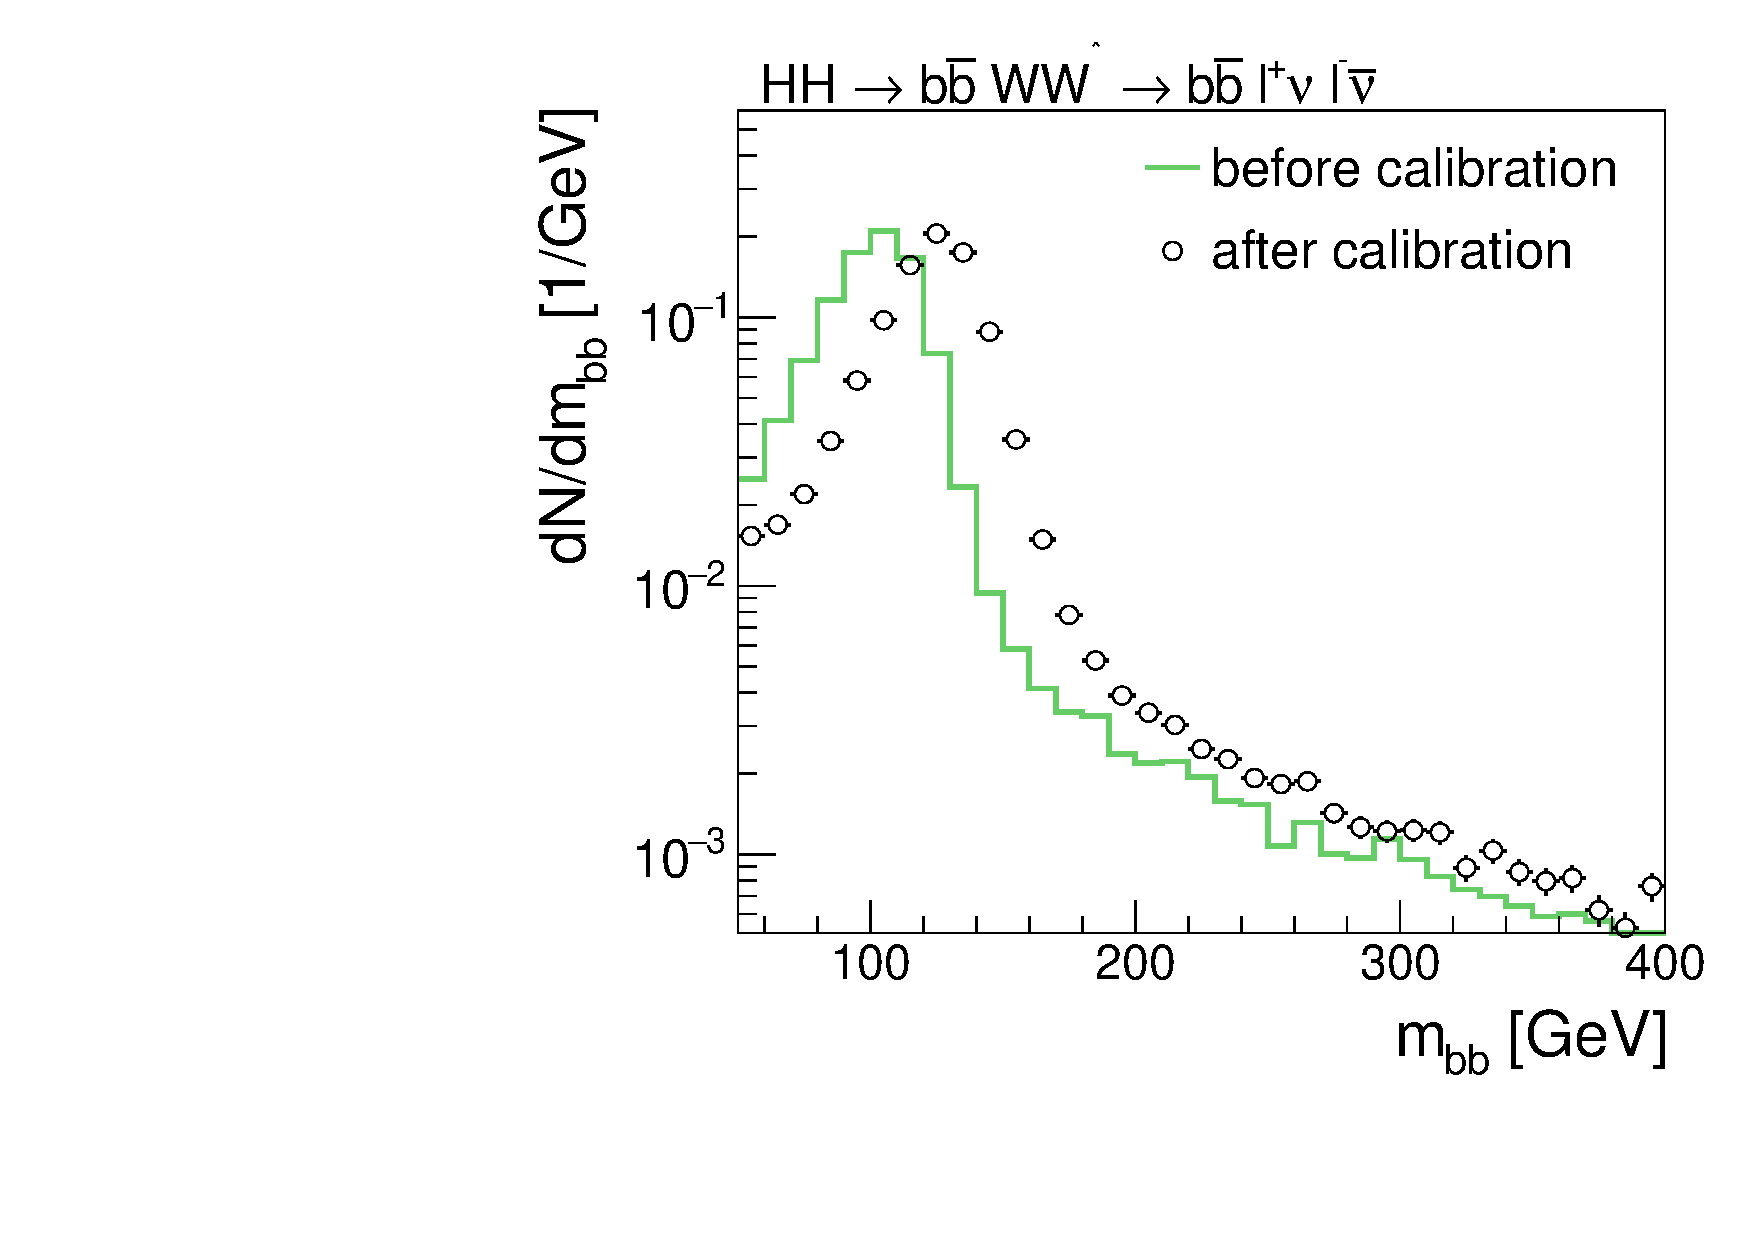
\includegraphics[width=0.48\textwidth]{plots/mbb_calibrated_vs_uncalibrated_signal.pdf}
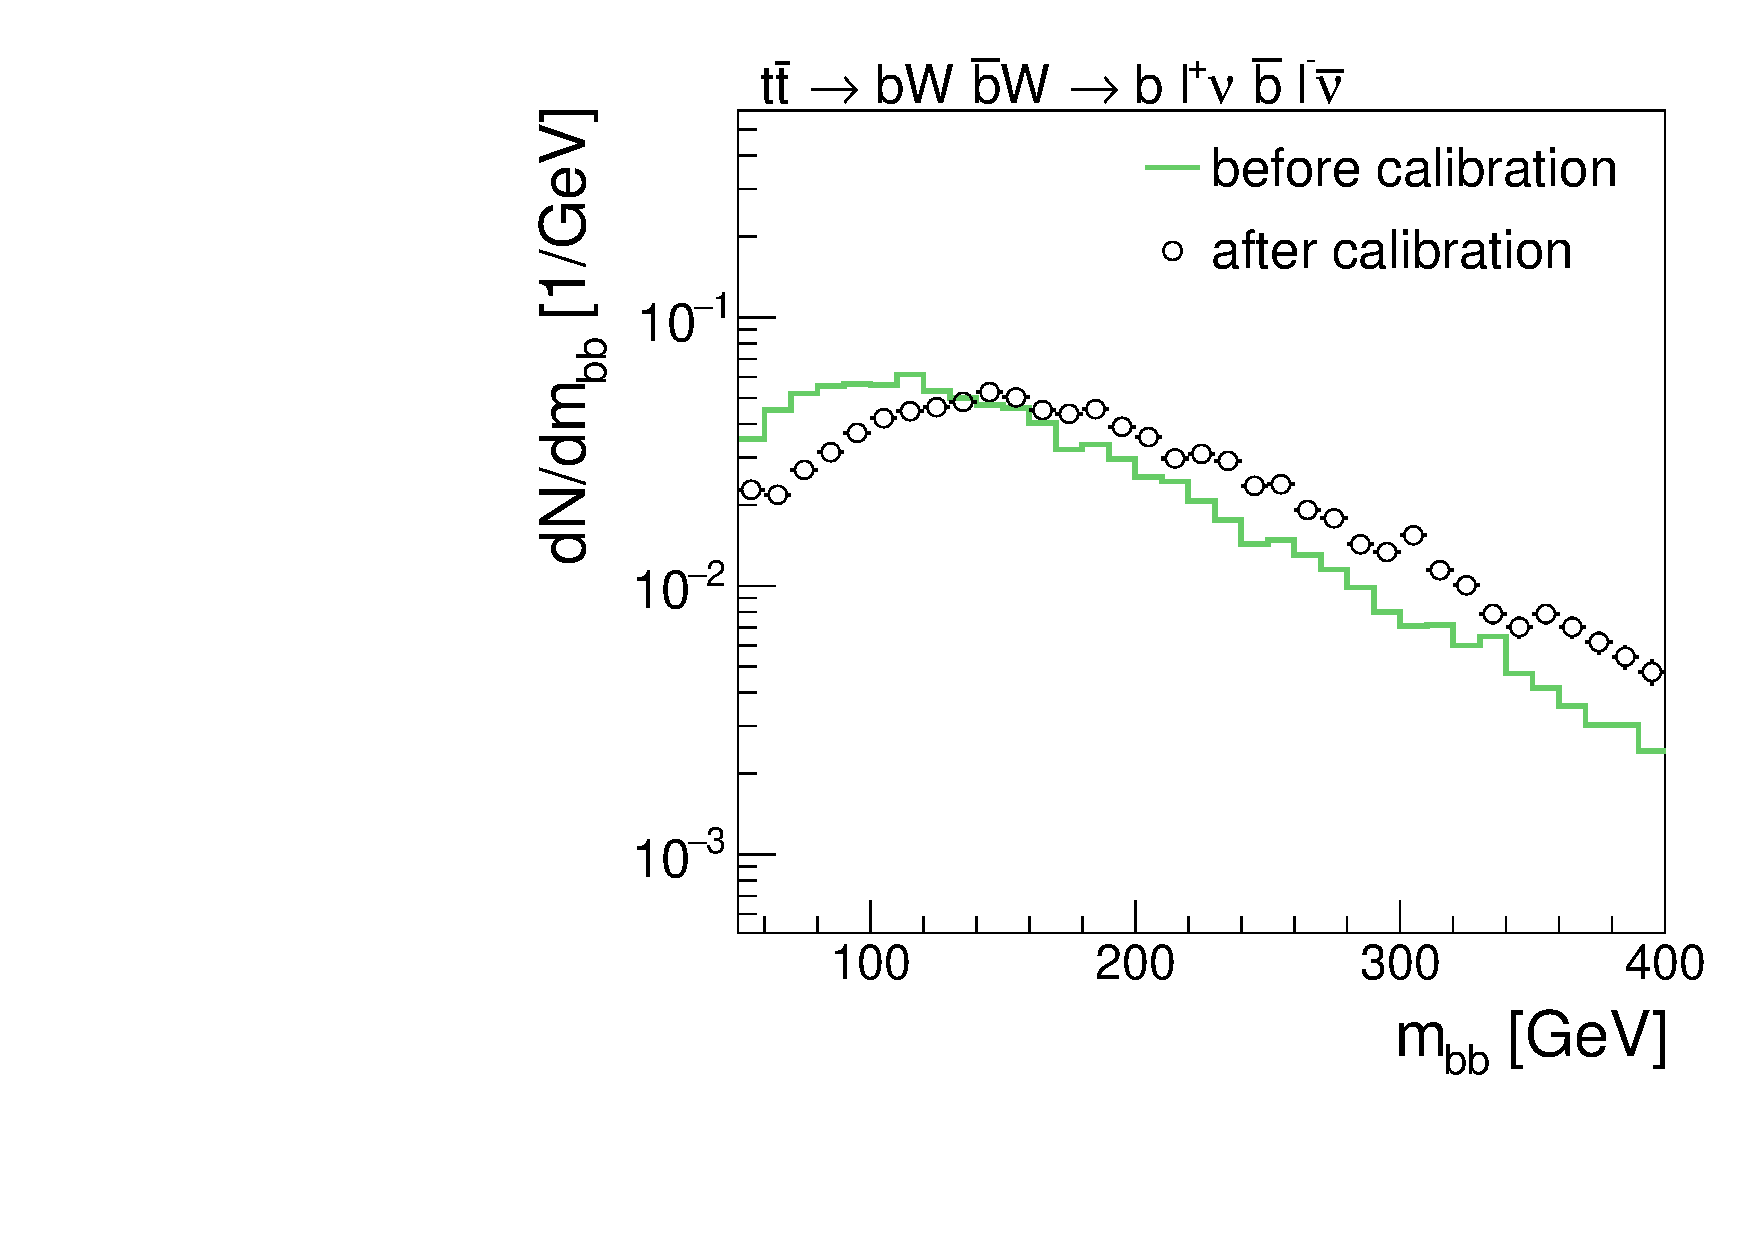
\includegraphics[width=0.48\textwidth]{plots/mbb_calibrated_vs_uncalibrated_background.pdf}
\fi
\caption{
  Distribution in $\mbb$, the mass of the two detector-level jets that are tagged as $\Pbottom$-jets,
  in $\dihiggs$ signal (left) and $\ttbar$ background (right) events before and after the jet energy calibration is applied.
}
\label{fig:mbb}
\end{figure}

Before we can compute the PDs $w_{0}(\vecy)$ and $w_{1}(\vecy)$ according to Eqs.~\ref{eq:mem_signal} and~\ref{eq:mem_background},
we need to determine the TF for the energy of $\Pbottom$-jets and for the transverse momentum components of the hadronic recoil
such that the TF match the experimental resolutions in the $\textsc{DELPHES}$ simulation.
We model the experimental resolution on the energy of $\Pbottom$-jets using a normal distribution:
\begin{linenowrapper}
\begin{equation}
W(E|\Ehat) = \frac{1}{\sqrt{2 \pi \sigma_{\Pbottom}^{2}}} \, e^{-\frac{(\pT - \pThat)^{2}}{2 \, \sigma_{\Pbottom}^{2}}} \, ,
\label{eq:resolution_b}
\end{equation}
\end{linenowrapper}
where $\pT = E \, \sin\theta$, $\pThat = \Ehat \, \sin\theta$, and $\theta$ refers to the polar angle of the jet.
The standard deviation $\sigma_{\Pbottom}$ depends on the jet energy and $\theta$.
We make the ansatz $\sigma_{\Pbottom} = k \cdot \sqrt{\Ehat \, \sin\theta}$ and determine the constant of proportionality $k$ such that it fits
the resolution on the energy of $\Pbottom$-jets in the $\textsc{DELPHES}$ simulation, yielding $k = 100\%$.
Our model for the jet energy resolution agrees with the resolution measured by the CMS collaboration during LHC Run $2$ that is shown in Fig.~3 of Ref.~\cite{JME-18-001}.
Our assumption that the polar angle $\theta$ of the jet is measured with negligible experimental resolution (\cf Section~\ref{sec:appendix_TF} of the appendix)
is justified by Fig.~5 of Ref.~\cite{JME-18-001}, which shows that the resolution on $\theta$ amounts to about $0.02$ radians for jets of $\pT = 25$~\GeV and decreases for jets of higher $\pT$.
The hadronic recoil $\rho$ is not directly available in the $\textsc{DELPHES}$ simulation.
To determine the resolution on $\rho$, we compute the transverse momentum components of the hadronic recoil by means of Eq.~\ref{eq:hadRecoil_true} at MC-truth
and by means of Eq.~\ref{eq:hadRecoil} at detector level.
The resolutions on $\pX^{\rho}$ and $\pY^{\rho}$ amount to $32.4$~\GeV for the $\dihiggs$ signal and to $30.3$~\GeV for the $\ttbar$ background.
The resolution on the energy of $\Pbottom$-jets is small compared to the resolution on the hadronic recoil,
which means that the resolution on the latter is dominated by the resolution on the $\vecMET$.
This allows us to compare the resolutions on $\pX^{\rho}$ and $\pY^{\rho}$ in the $\textsc{DELPHES}$ simulation to published $\vecMET$ resolutions during LHC Run $2$.
The $\vecMET$ resolution for simulated $\ttbar$ events in the ATLAS detector is shown in Fig.~9 of Ref.~\cite{ATLAS:2018txj} and amounts to $25$-$30$~\GeV,
similar to what we find with $\textsc{DELPHES}$ for the CMS detector (we did not find numbers published by CMS for the $\vecMET$ resolution in $\ttbar$ events during LHC Run $2$).
We assume that the resolutions on $\pX^{\rho}$ and $\pY^{\rho}$ are uncorrelated and the same for signal and background events.
Thus, we use:
\begin{linenowrapper}
\begin{equation}
V = \sigma_{\rho}^{2} \cdot I_{2} 
\label{eq:resolution_rho}
\end{equation}
\end{linenowrapper}
with $\sigma_{\rho} = 31.4$~\GeV for when computing the PDs $w_{0}(\vecy)$ and $w_{1}(\vecy)$ for $\dihiggs$ signal and $\ttbar$ background events.

With these TF, we can proceed to compute the PDs $w_{0}(\vecy)$ and $w_{1}(\vecy)$.
Distributions in $w_{0}(\vecy)$ and $w_{1}(\vecy)$ for $\dihiggs$ signal and $\ttbar$ background events are shown in Fig.~\ref{fig:probS_and_probB}.
The axis of abscissae is drawn in logarithmic scale to better visualize small values of the PDs.
The PDs are computed at MC-truth and at detector level.
When computing the PDs at MC-truth level, 
we set the ``measured'' momenta of electrons and muons to their generator-level values, the ``measured'' momenta of the $\Pbottom$-jets to the momenta of the corresponding parton-level bottom quarks,
and the ``measured'' transverse momentum components of the hadronic recoil to their true values $\pXhat^{\rho}$ and $\pYhat^{\rho}$.
The latter are computed according to Eq.~\ref{eq:hadRecoil_true}.
We also demand that both $\Pbottom$-jets are matched, within a cone of size $\delta R = 0.3$,
to bottom quarks that originate from either $\PHiggs$ boson or from top quark decays when we compute the PDs at MC-truth level.
The same TF, described in the previous paragraph, are used when computing the PDs $w_{0}(\vecy)$ and $w_{1}(\vecy)$ at MC-truth and at detector level.
The distributions in the PDs for the ``correct'' hypothesis ($w_{0}(\vecy)$ for signal and $w_{1}(\vecy)$ for background events)
peak close to one and fall rapidly towards smaller values, while the distributions in the PDs for the ``wrong'' hypothesis
($w_{1}(\vecy)$ for signal and $w_{0}(\vecy)$ for background events)
exhibit more pronounced tails towards small values.
Interestingly, the distributions in the PDs for the wrong hypothesis change only by a small amount between MC-truth and detector level.
The main effect of the experimental resolutions on the energy of $\Pbottom$-jets and on the transverse momentum of the hadronic recoil
as well as of the misidentification of light quark or gluon jets as $\Pbottom$-jets is to increase the tail towards small values for the distributions in the PDs for the correct hypothesis.

\begin{figure}
\ifx\ver\verPreprint
\setlength{\unitlength}{1mm}
\begin{center}
\begin{picture}(160,144)(0,0)
\put(-1.0, 78.0){\mbox{\includegraphics*[height=66mm]
 {plots/effectOfFakes_2histograms_probS_signal.pdf}}}
\put(80.0, 78.0){\mbox{\includegraphics*[height=66mm]
 {plots/effectOfFakes_2histograms_probS_background.pdf}}}
\put(-1.0, 0.0){\mbox{\includegraphics*[height=66mm]
 {plots/effectOfFakes_2histograms_probB_signal.pdf}}}
\put(80.0, 0.0){\mbox{\includegraphics*[height=66mm]
 {plots/effectOfFakes_2histograms_probB_background.pdf}}}
\end{picture}
\end{center}
\fi
\ifx\ver\verPAPER
\centering
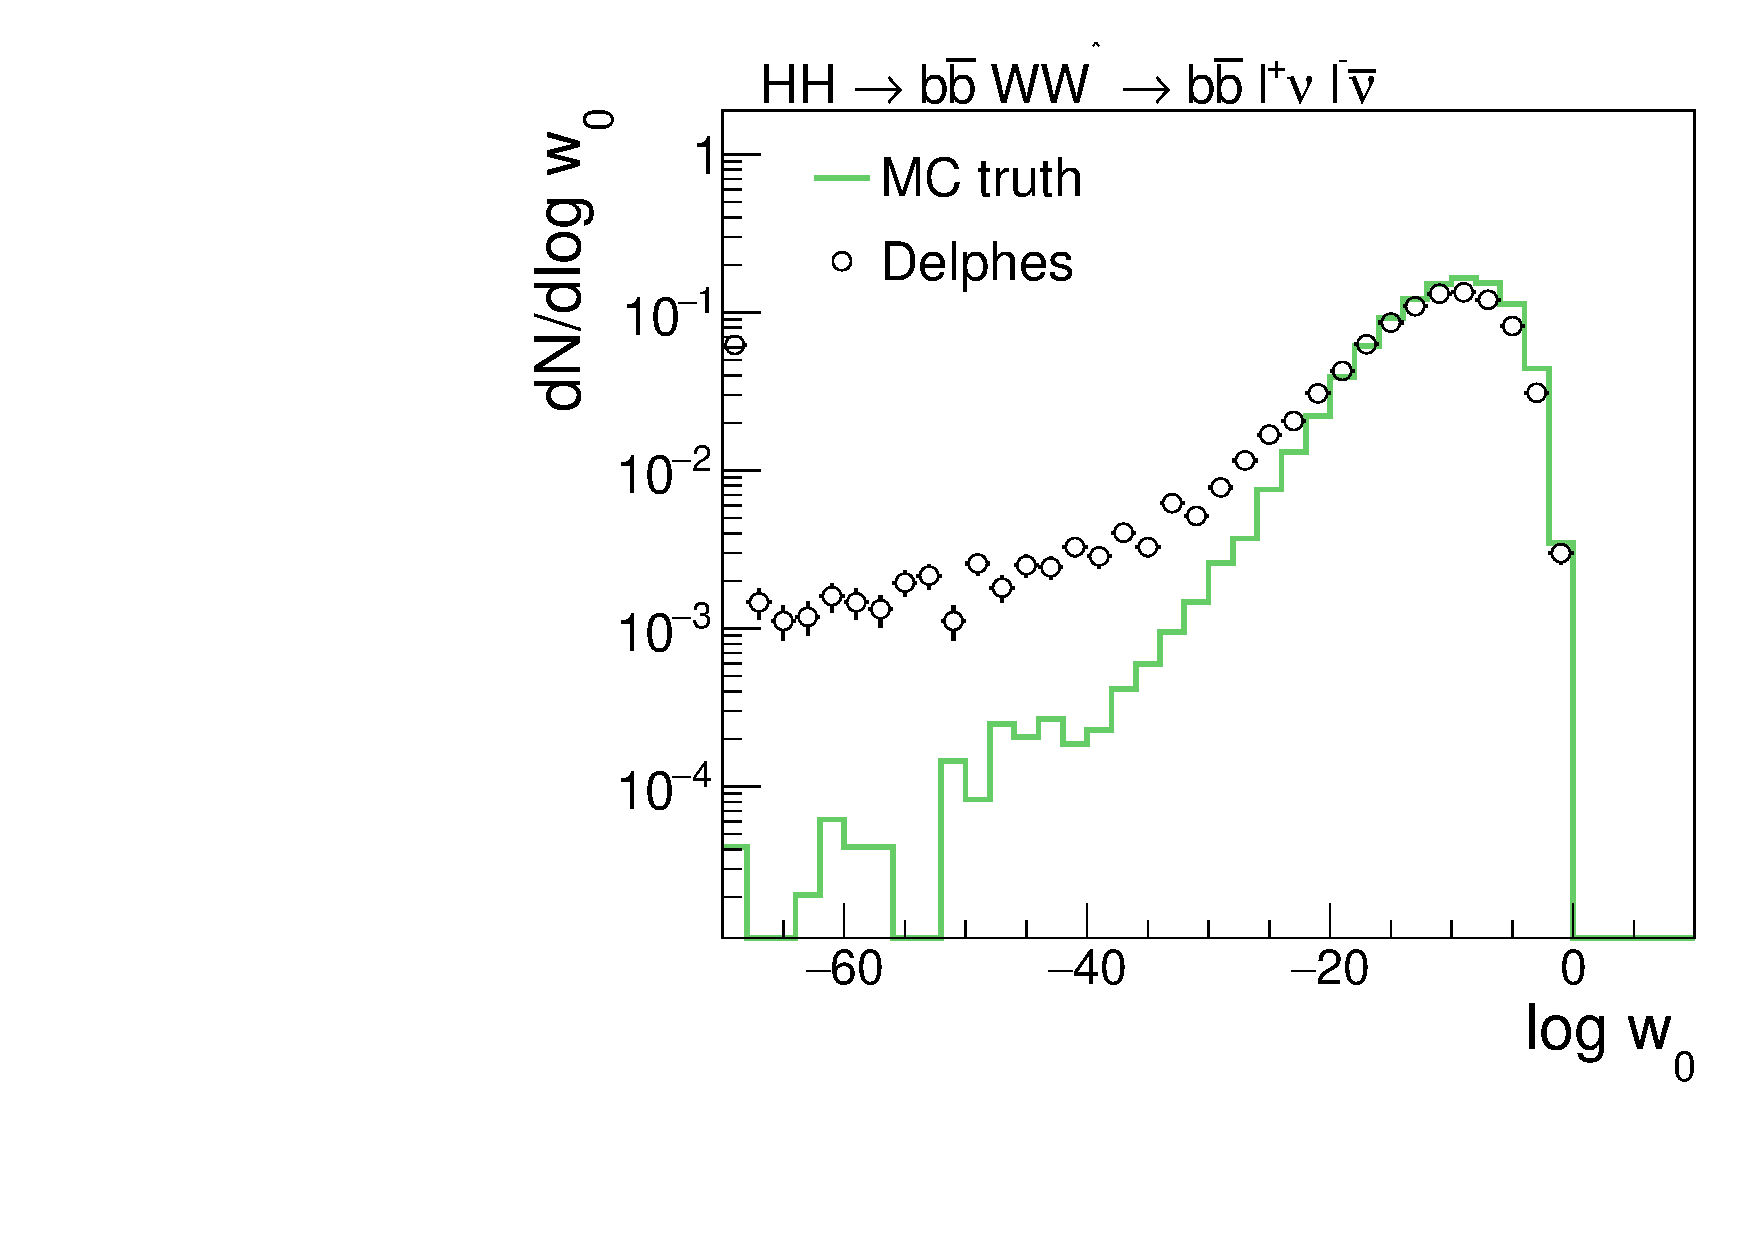
\includegraphics[width=0.48\textwidth]{plots/makePlotsForPaper_delphes_vs_mctruth_probS_signal.pdf}
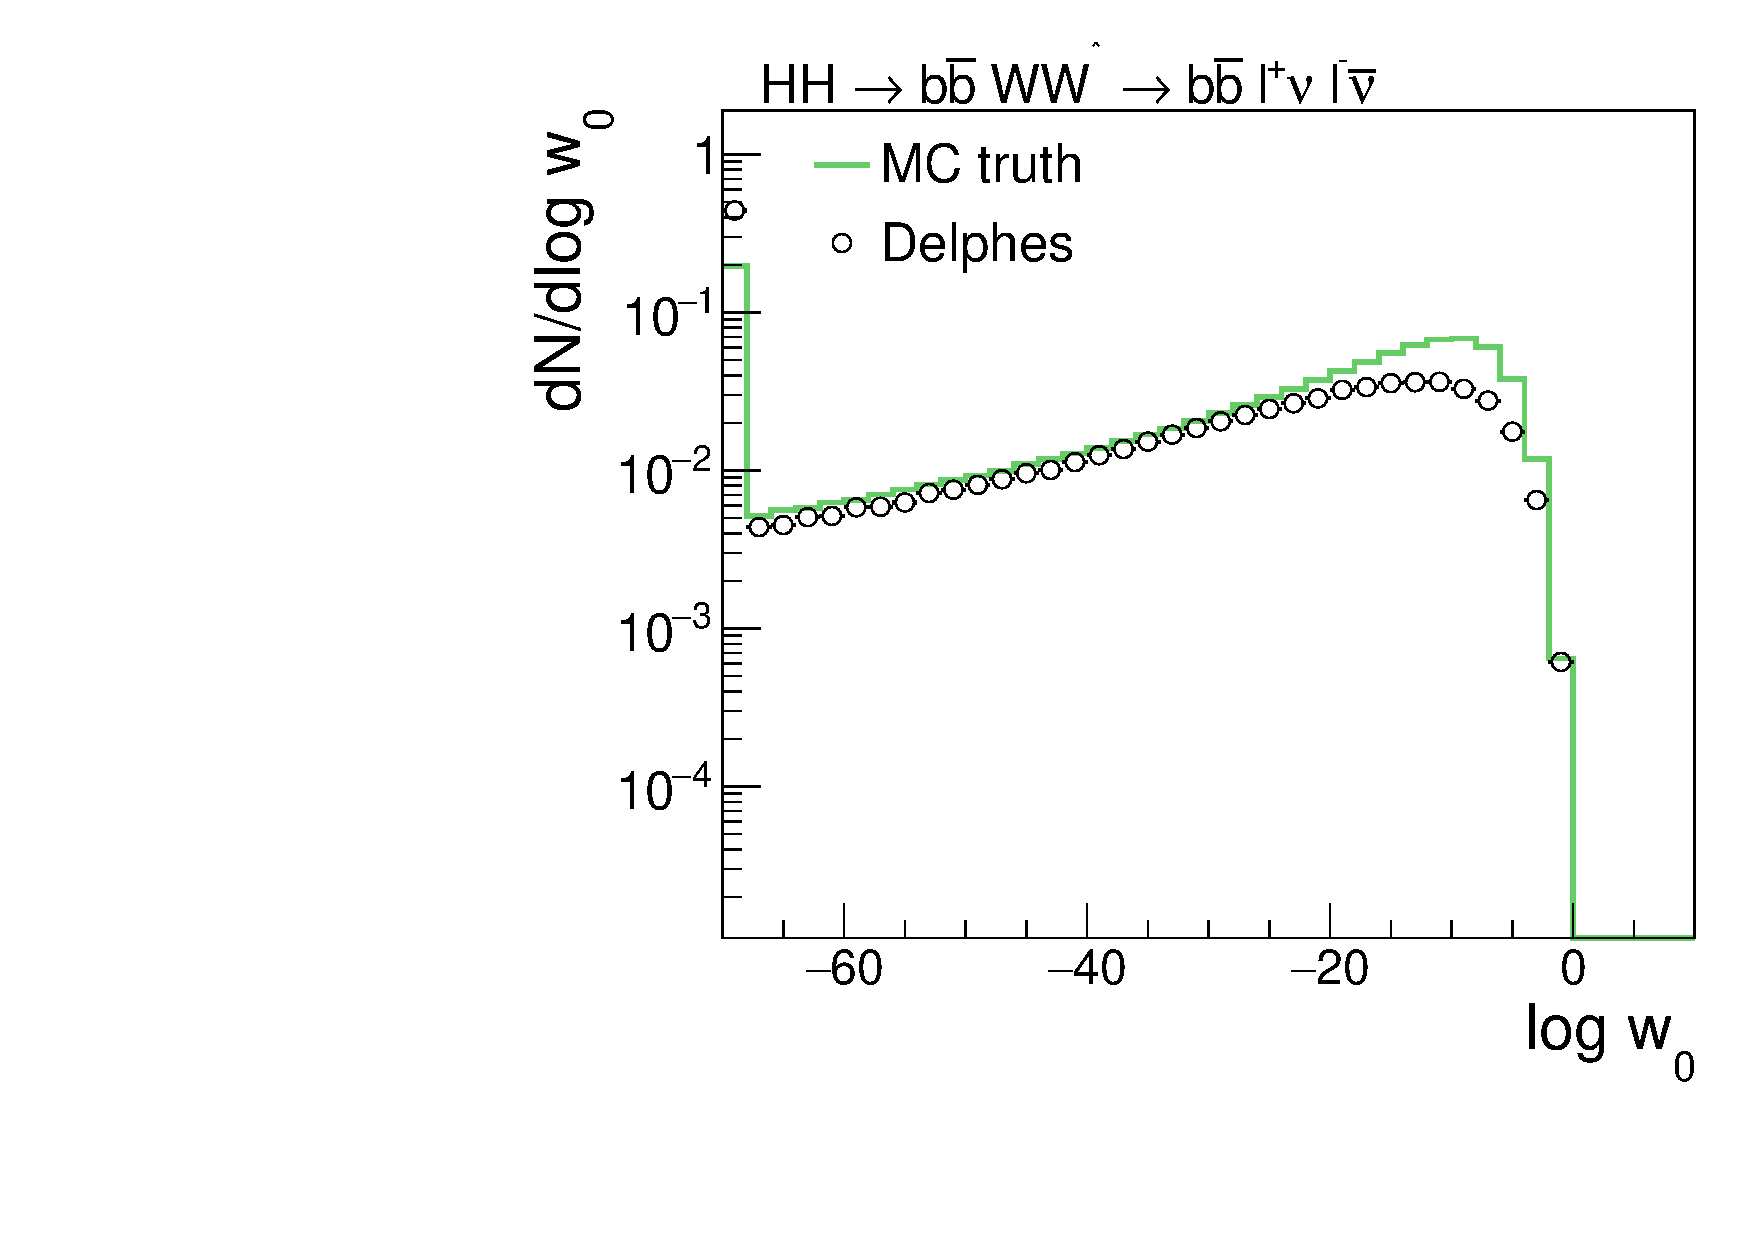
\includegraphics[width=0.48\textwidth]{plots/makePlotsForPaper_delphes_vs_mctruth_probS_background.pdf}
\hspace{0.04\textwidth}
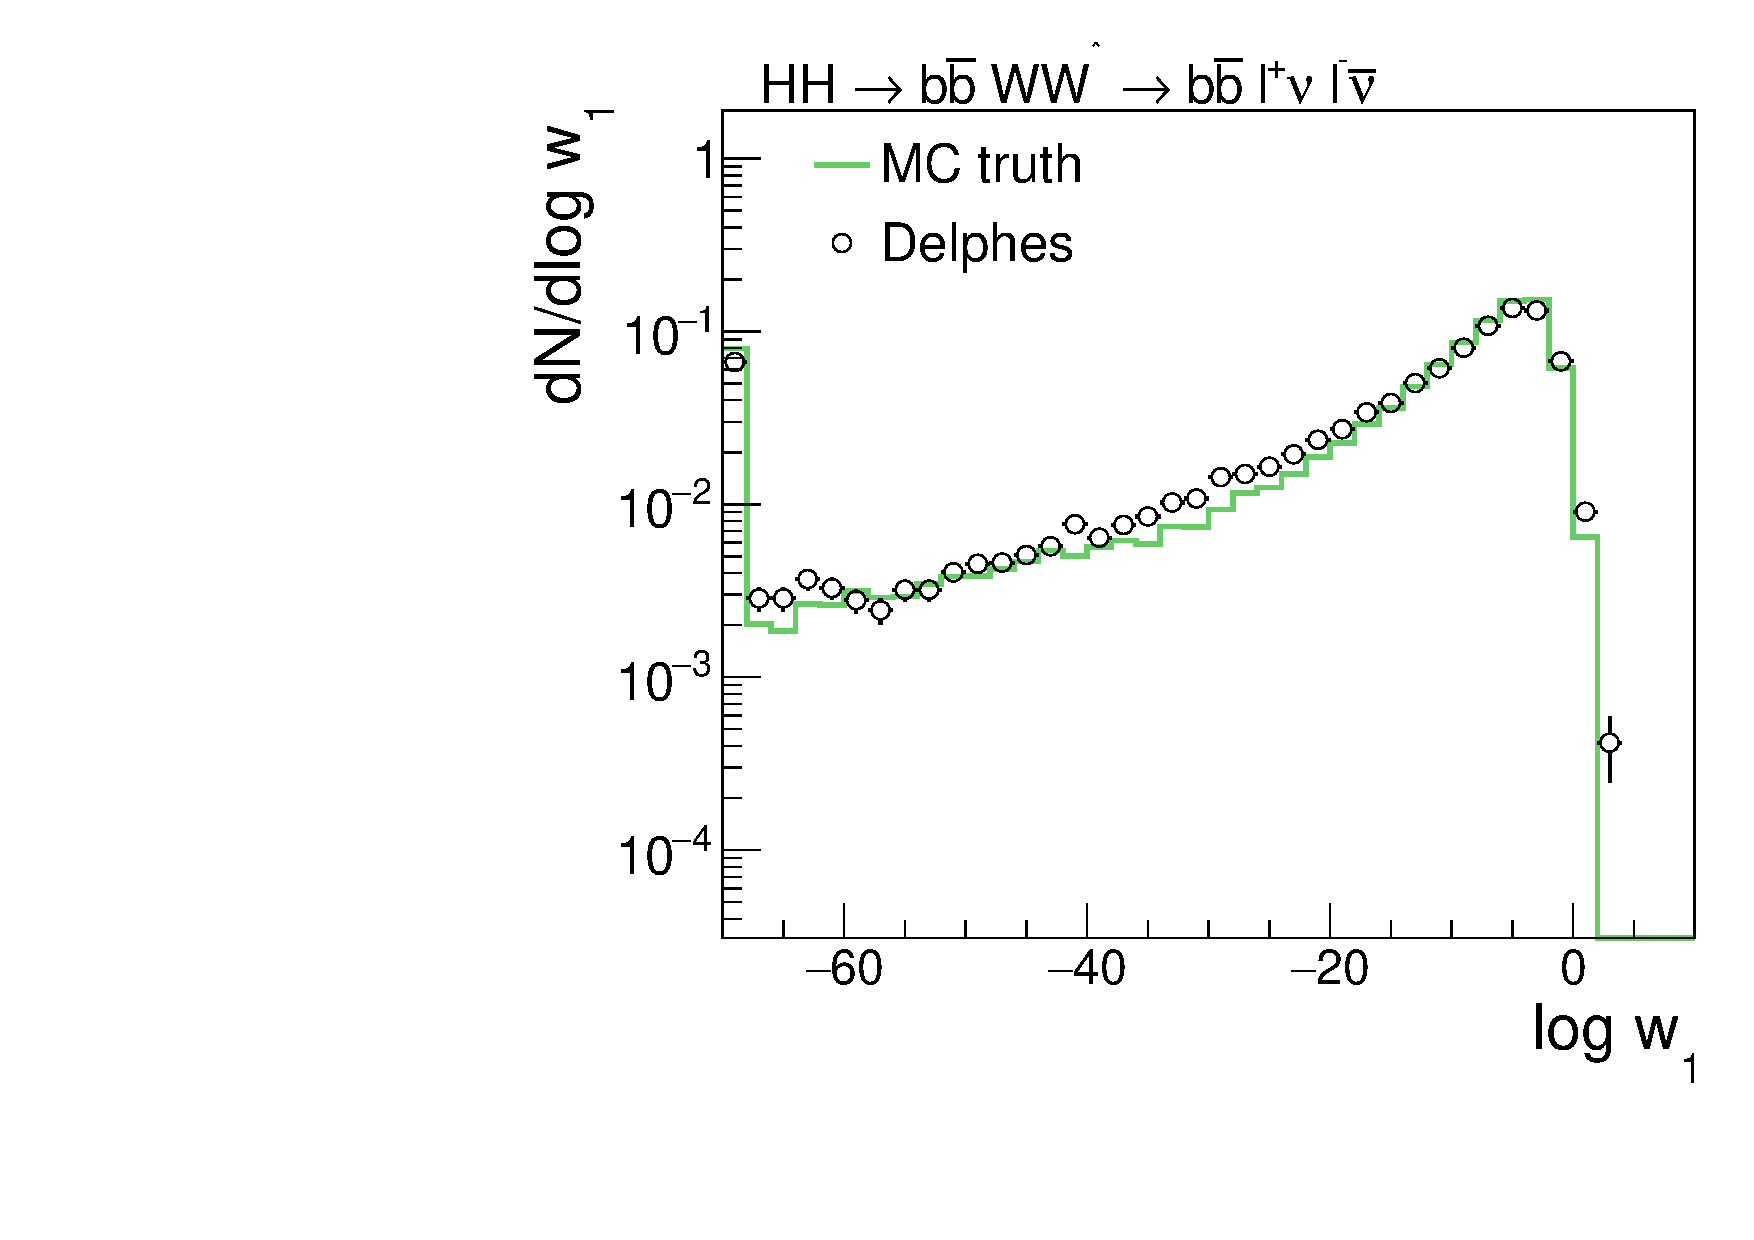
\includegraphics[width=0.48\textwidth]{plots/makePlotsForPaper_delphes_vs_mctruth_probB_signal.pdf}
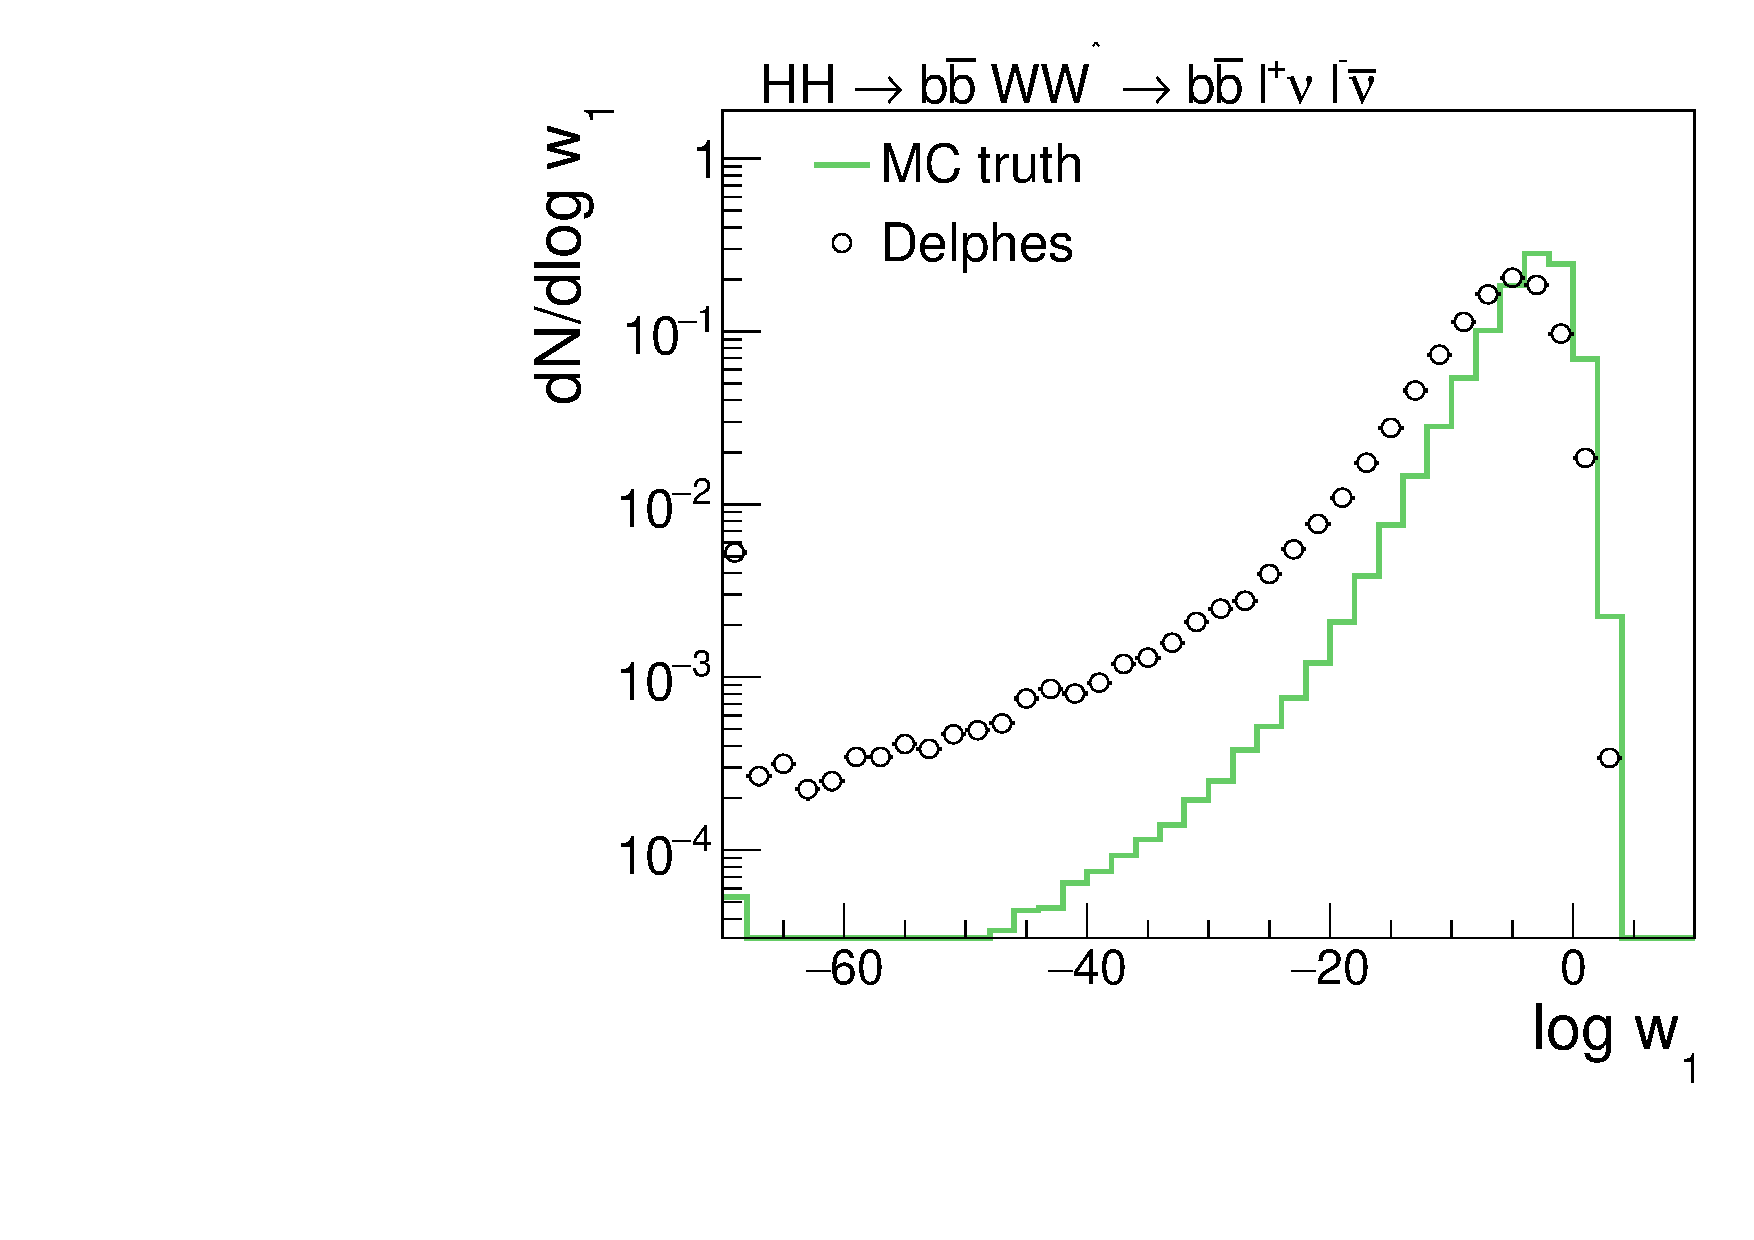
\includegraphics[width=0.48\textwidth]{plots/makePlotsForPaper_delphes_vs_mctruth_probB_background.pdf}
\fi
\caption{
  Distributions in the PDs $w_{0}(\vecy)$ (upper) and $w_{1}(\vecy)$ (lower), computed according to Eqs.~\ref{eq:mem_signal} and~\ref{eq:mem_background},
  for $\dihiggs$ signal (left) and $\ttbar$ background (right) events.
  The PDs are computed at MC-truth and at detector level.
}
\label{fig:probS_and_probB}
\end{figure}

The corresponding distributions in the LR $P(\vecy)$, computed according to Eq.~\ref{eq:memLR}, are shown in Fig.~\ref{fig:memLR}.
Signal events are characterized by high values of $P(\vecy)$, while background events typically have low values.
The secondary peak of the distribution at low values for $\dihiggs$ signal (at high values for $\ttbar$ background) events
is due to events in which the event kinematics are atypical for signal (background) events, 
resulting in the PD for the wrong hypothesis $w_{1}(\vecy)$ ($w_{0}(\vecy)$) to be higher than the PD for the correct hypothesis $w_{0}(\vecy)$ ($w_{1}(\vecy)$).
About $4\%$ of signal ($10\%$ of background) events populate the leftmost (rightmost) bin of the distribution in the LR $P(\vecy)$ in case $P(\vecy)$ is computed at MC-truth level.
In case the LR $P(\vecy)$ is computed at detector level, the fraction of $\dihiggs$ signal ($\ttbar$ background) events 
that populate the leftmost (rightmost) bin increases to $14\%$ (decreases to $7\%$).
The ``receiver-operating-characteristic'' (ROC) curves~\cite{ROCcurve} that correspond to these distributions are shown in Fig.~\ref{fig:ROC}.
The ROC curve quantifies the separation between the $\dihiggs$ signal and the $\ttbar$ background
and is obtained by varying the threshold of a cut on the LR $P(\vecy)$ and plotting the fractions of signal and background events passing the cut.
For a signal efficiency of $35\%$, the $\ttbar$ background is reduced by almost three orders of magnitude, to a level of $1.2$ permille, in case the LR $P(\vecy)$ is computed at MC-truth level.
In case the LR $P(\vecy)$ is computed at detector level, the $\ttbar$ background is reduced to a level of $2.6$ permille.
The main reason for the degradation in separating the $\dihiggs$ signal from the $\ttbar$ background that occurs at detector level
are signal events in which one of the bottom quarks originating from the $\PHiggs$ boson decay is not reconstructed as $\Pbottom$-jet at detector level
and a light quark or gluon jet is misidentified as $\Pbottom$-jet instead.
If this happens, the mass of the two detector-level jets that are reconstructed as $\Pbottom$-jets are often incompatible with $m_{\PHiggs}$.
The presence of a BW propagator in the ME $\mathcal{M}_{0}(\vecphat)$ for the signal hypothesis,
which enforces that the mass of the pair of $\Pbottom$-jets equals $m_{\PHiggs}$,
introduces large ``pulls'' in the TF $W(E|\Ehat)$ for the $\Pbottom$-jet energy in this case, which diminish the value of the integrand.
To better gauge the separation of the $\dihiggs$ signal from the $\ttbar$ background achieved by the LR $P(\vecy)$,
we compute signal efficiencies and background rates that one would obtain by cutting on the mass $\mbb$ of the $\Pbottom$-jet pair, shown in Fig.~\ref{fig:mbb}, for comparison.
Fitting the peak of the distribution in $\mbb$ obtained after the jet calibration is applied in $\dihiggs$ signal events
with a normal distribution yields a mean of $119.4$~\GeV and a standard deviation of $20.5$~\GeV.
Selecting events for which the mass $\mbb$ is within $1$ ($2$) standard deviations around the mean
keeps $68.9\%$ ($86.9\%$) of the $\dihiggs$ signal and $22.1\%$ ($40.6\%$) of the $\ttbar$ background.
The mass $\mbb$ is presumably one of the most powerful single observable to separate the $\dihiggs$ signal from the $\ttbar$ background.
The conclusion that we draw from the numbers quoted in this paragraph is that by exploiting the full difference in event kinematics between the $\dihiggs$ signal and the $\ttbar$ background with the MEM
one can significantly improve the separation of the $\dihiggs$ signal from the $\ttbar$ background compared to imposing simple cuts on single observables.
We remark that the misidentification of hadrons as leptons is not simulated in $\textsc{DELPHES}$ and hence not accounted for in the detector-level ROC curve shown in Fig.~\ref{fig:ROC}.
We expect this have only a small effect on the ROC curve,
as analysis of $\dihiggs$ production performed by the CMS collaboration in the decay channel $\Pbottom\APbottom\PW\PW\virt$ in LHC Run $2$
found the misidentification of hadrons as leptons to constitute only a small, if not negligible, source of background.

\begin{figure}
\ifx\ver\verPreprint
\setlength{\unitlength}{1mm}
\begin{center}
\begin{picture}(160,66)(0,0)
\put(-1.0, 0.0){\mbox{\includegraphics*[height=66mm]
 {plots/makePlotsForPaper_delphes_vs_mctruth_memLR_signal.pdf}}}
\put(80.0, 0.0){\mbox{\includegraphics*[height=66mm]
 {plots/makePlotsForPaper_delphes_vs_mctruth_memLR_background.pdf}}}
\end{picture}
\end{center}
\fi
\ifx\ver\verPAPER
\centering
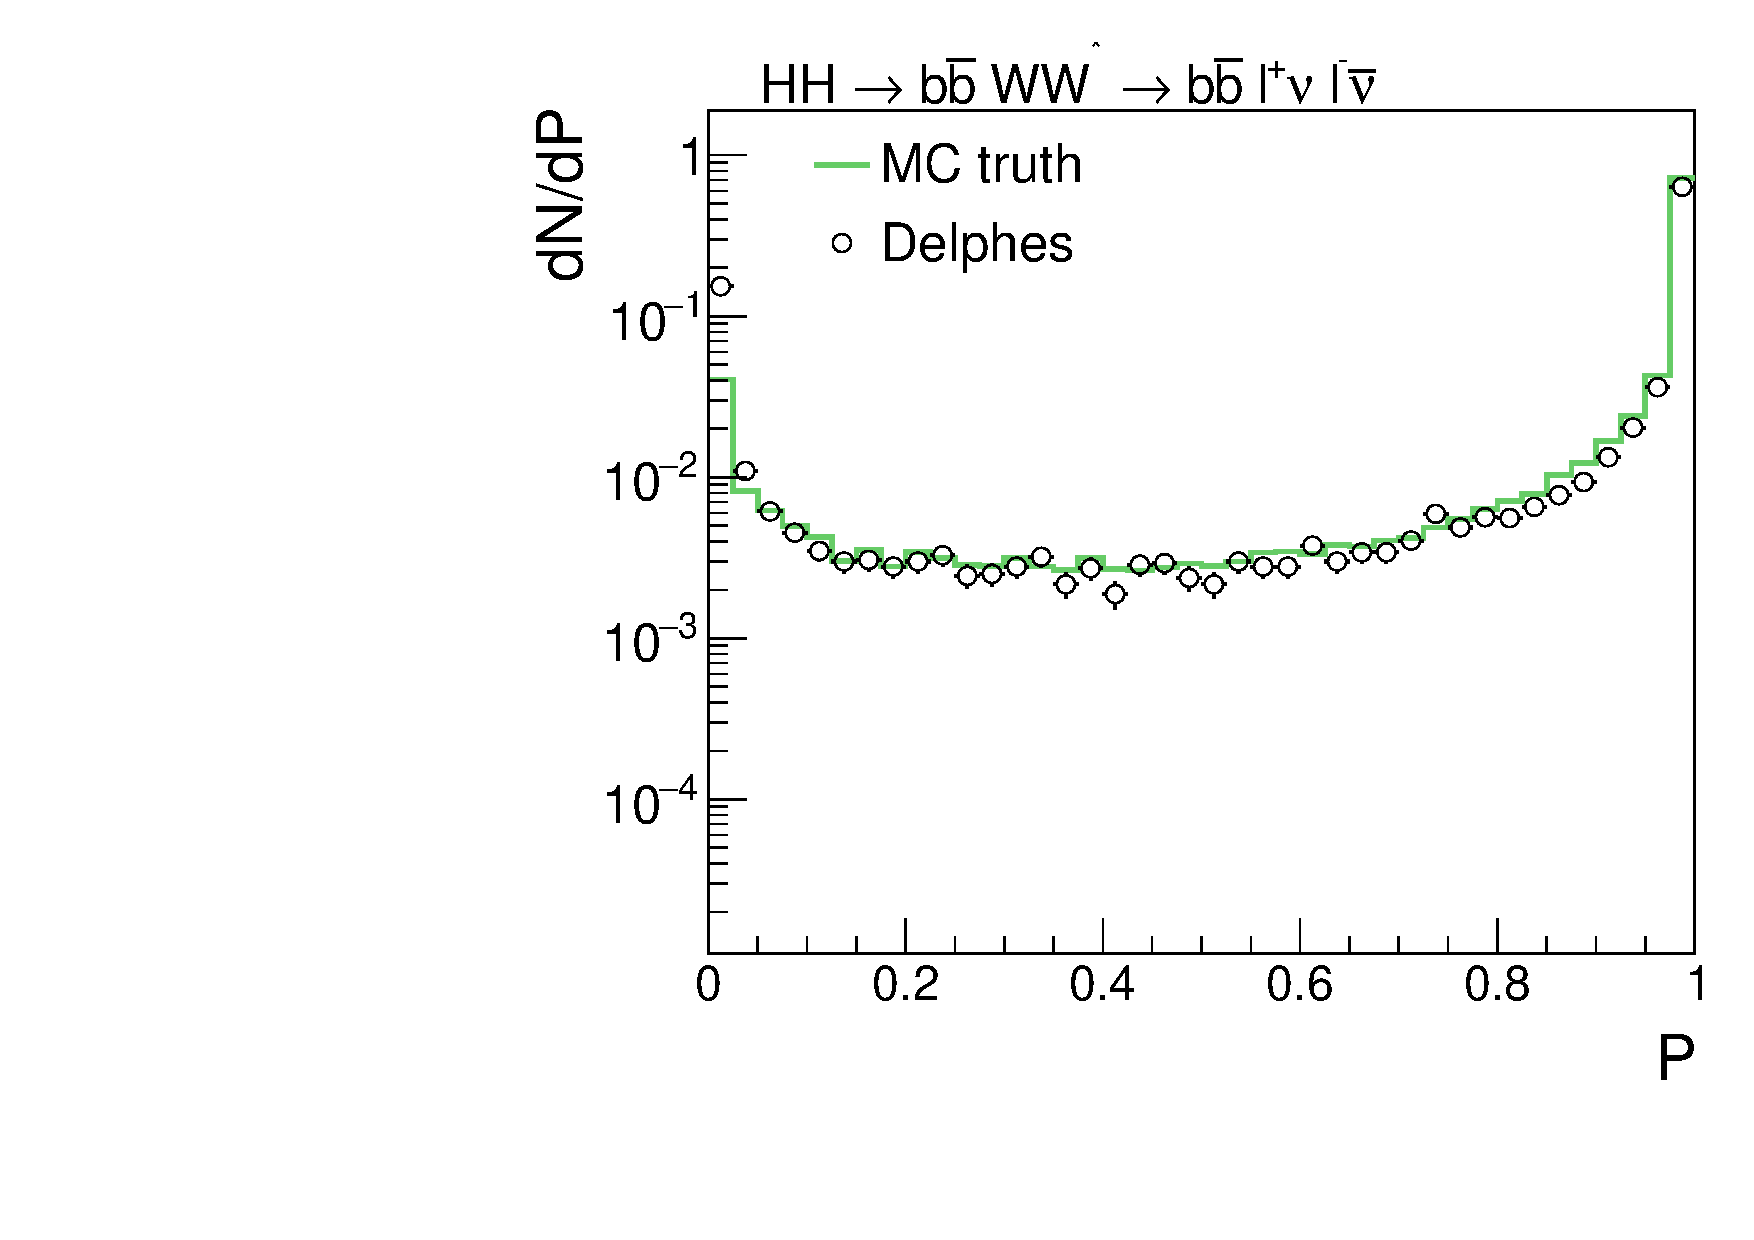
\includegraphics[width=0.48\textwidth]{plots/makePlotsForPaper_delphes_vs_mctruth_memLR_signal.pdf}
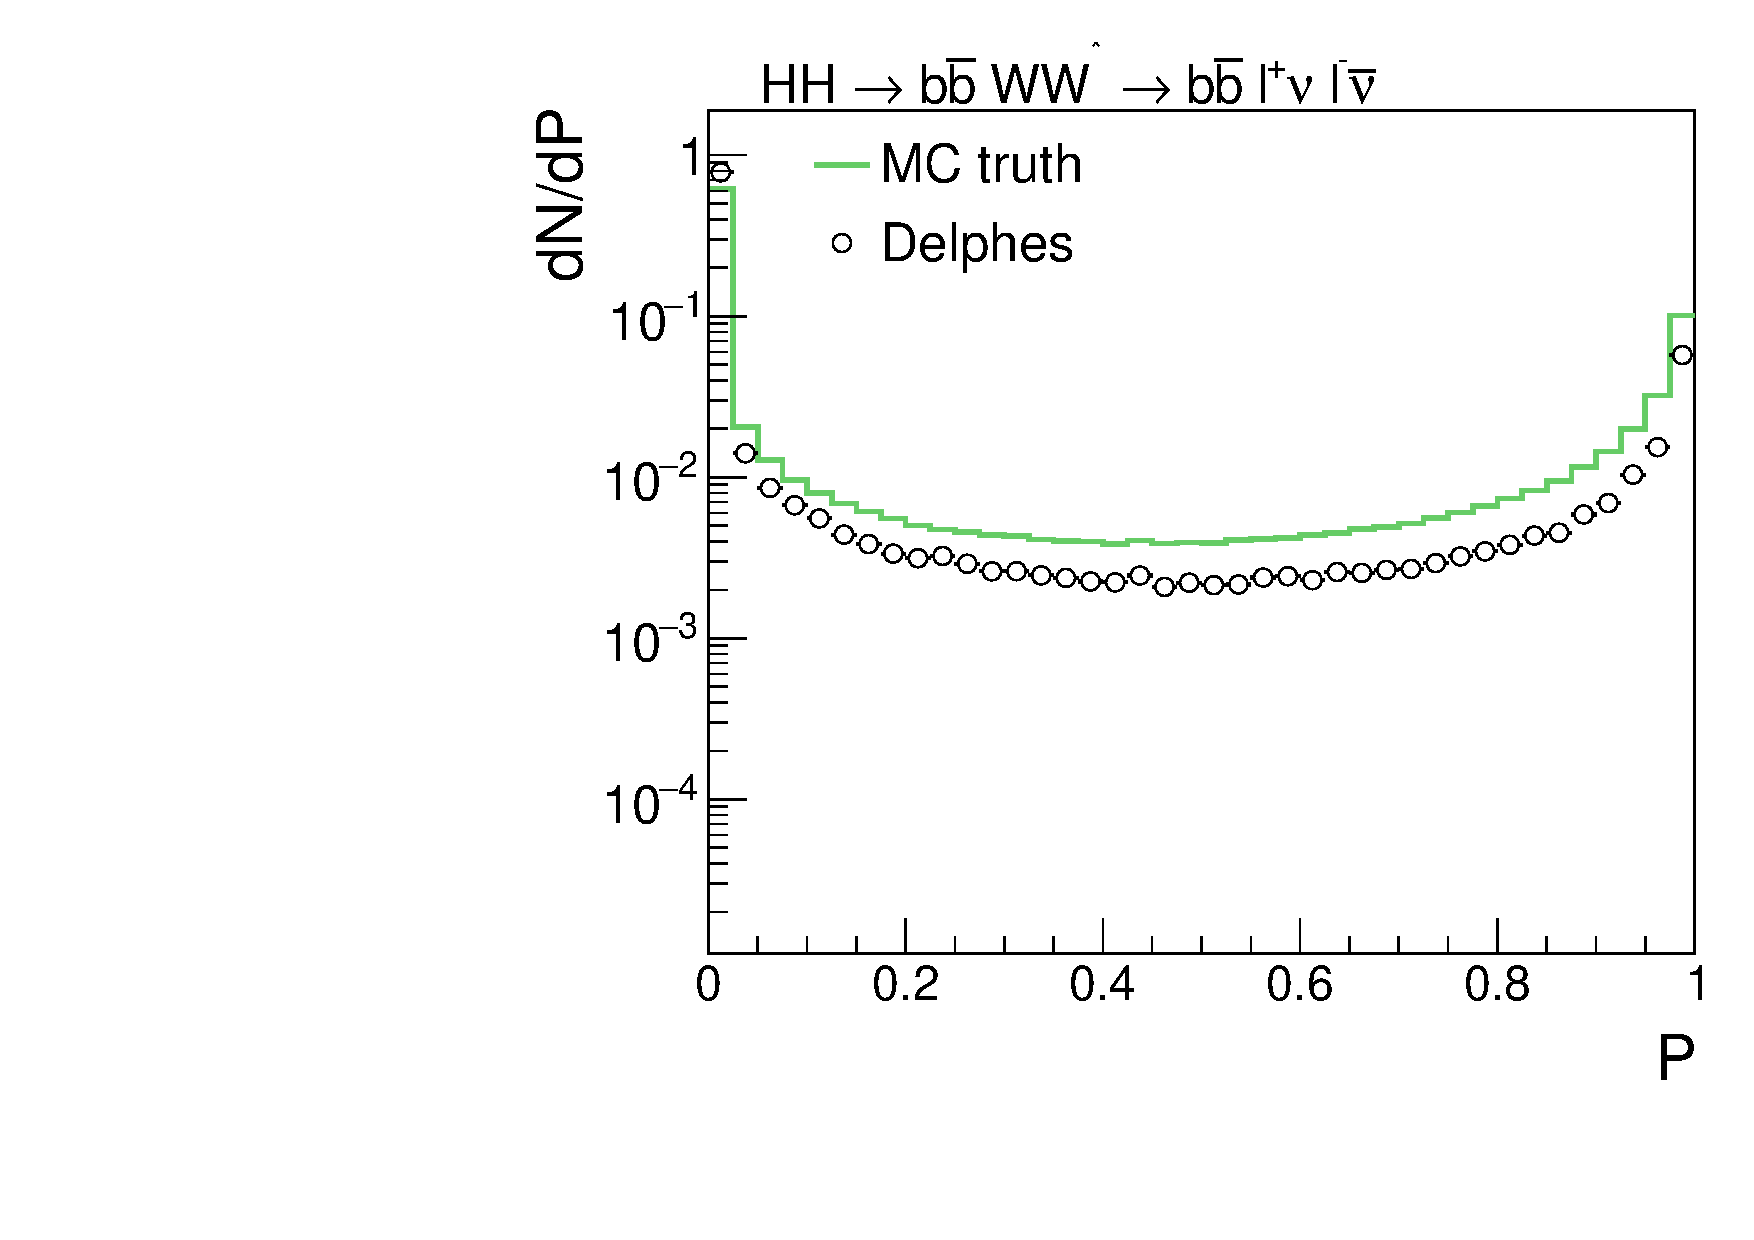
\includegraphics[width=0.48\textwidth]{plots/makePlotsForPaper_delphes_vs_mctruth_memLR_background.pdf}
\fi
\caption{
  Distributions in the LR $P(\vecy)$, computed according to Eq.~\ref{eq:memLR},
  for $\dihiggs$ signal (left) and $\ttbar$ background (right) events.
  The LR $P(\vecy)$ is computed using the PDs $w_{0}(\vecy)$ and $w_{1}(\vecy)$ shown in Fig.~\ref{fig:probS_and_probB} as input
  and is computed at MC-truth and at detector level.
}
\label{fig:memLR}
\end{figure}

\begin{figure}
\ifx\ver\verPreprint
\setlength{\unitlength}{1mm}
\begin{center}
\begin{picture}(160,78)(0,0)
\put(39.5, 0.0){\mbox{\includegraphics*[height=78mm]
 {plots/makePlotsForPaper_delphes_vs_mctruth_ROC.pdf}}}
\end{picture}
\end{center}
\fi
\ifx\ver\verPAPER
\centering
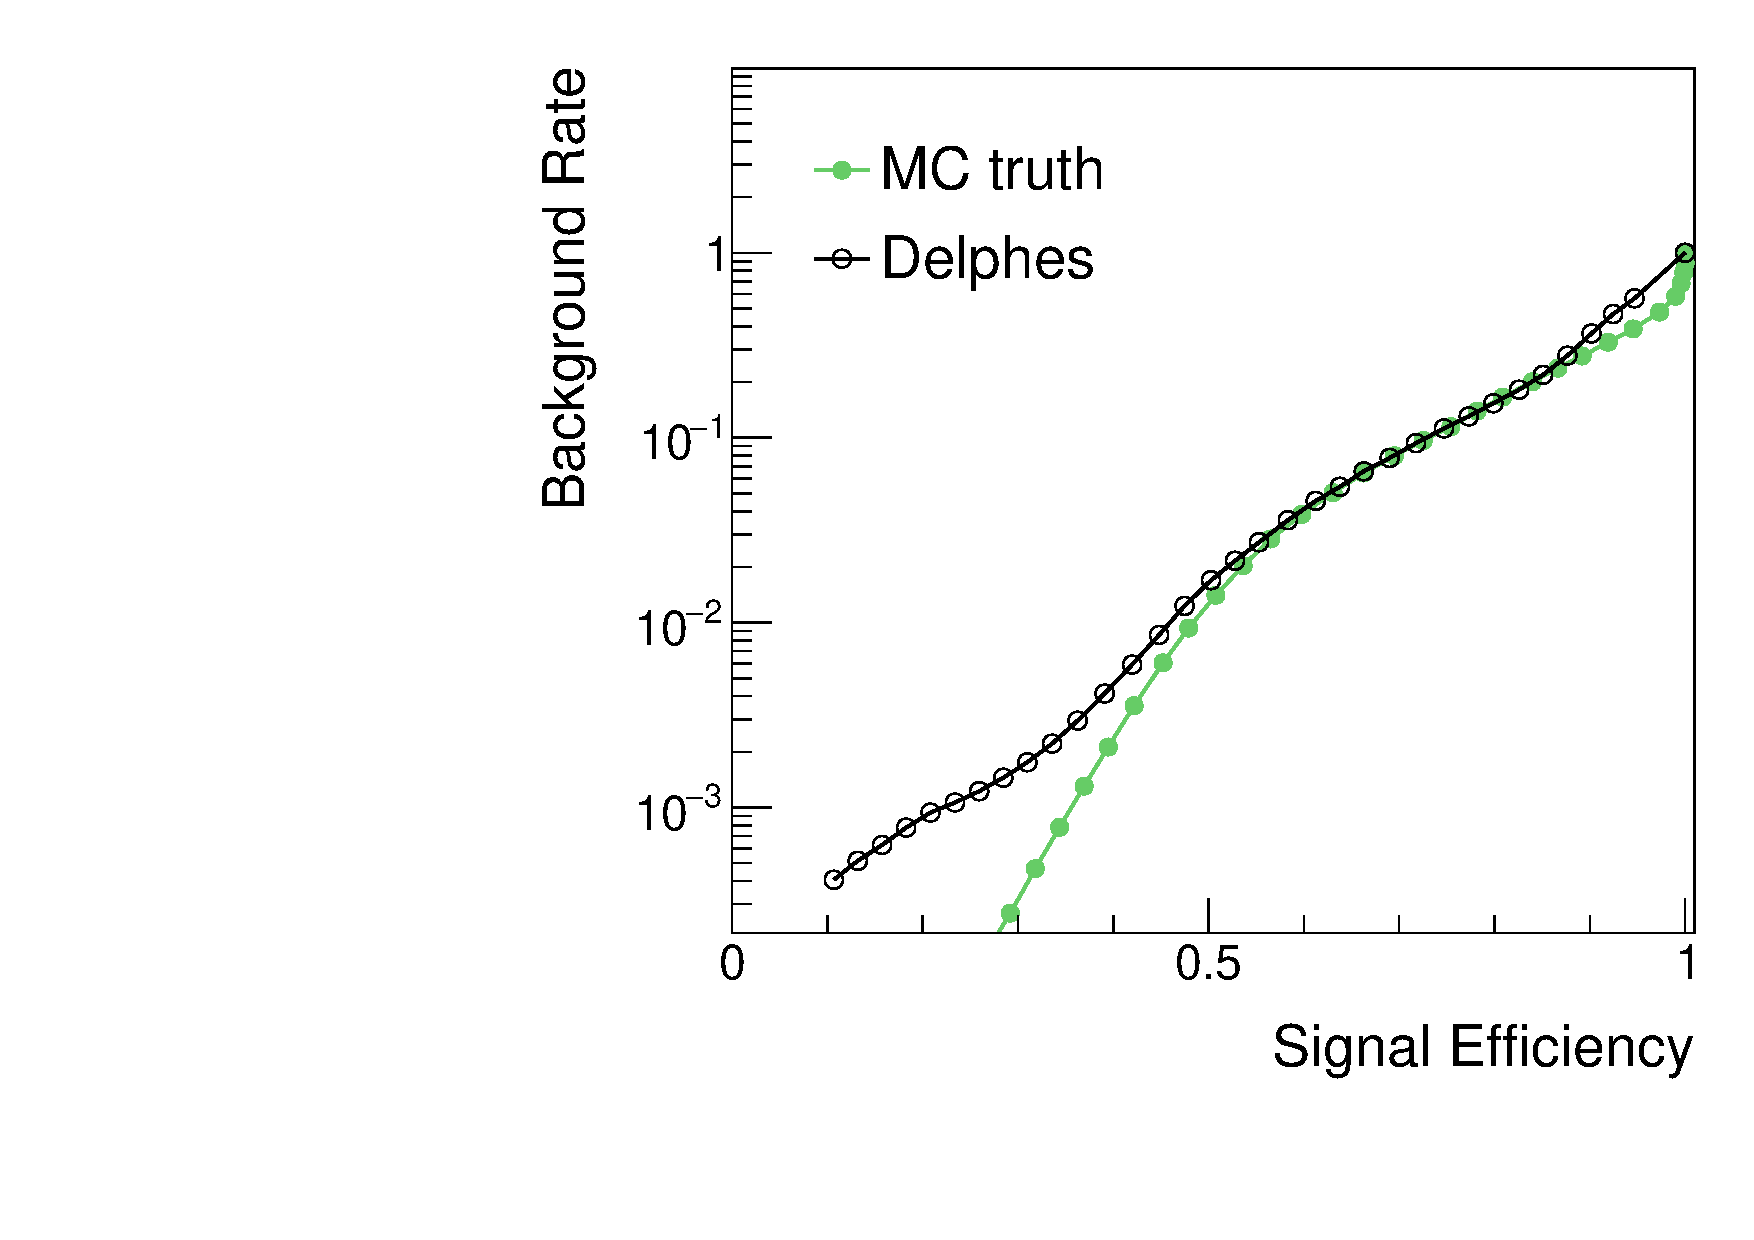
\includegraphics[width=0.48\textwidth]{plots/makePlotsForPaper_delphes_vs_mctruth_ROC.pdf}
\fi
\caption{
  Graphs of background rate versus signal efficiency (``ROC curve''), at MC-truth and at detector level,
  obtained by applying a cut on the distributions in the likelihood ratios $P(\vecy)$ shown in Fig.~\ref{fig:memLR}.
}
\label{fig:ROC}
\end{figure}

We conclude this section with an estimate of the effect of using LO ME when computing the weights $w_{0}(\vecy)$ and $w_{1}(\vecy)$ 
by means of Eqs.~(\ref{eq:mem_signal}) and~(\ref{eq:mem_background}) and of the computing-time requirements of the MEM.
Unfortunately, we cannot compare the performance of the MEM
for the case of using ME generated at LO versus ME generated at NLO in Eqs.~(\ref{eq:mem_signal}) and~(\ref{eq:mem_background}) directly,
because the program $\textsc{MadGraph\_aMCatNLO}$ does not support the generation of code for NLO ME at present
and also because the usage of NLO ME in the MEM would increase the computing-time requirements by $1$-$2$ orders of magnitude.
Instead, we use ME generated at LO accuracy in Eqs.~(\ref{eq:mem_signal}) and~(\ref{eq:mem_background}) 
and compare the resulting performance in separating the $\dihiggs$ signal from the $\ttbar$ background
for MC samples simulated at LO and at NLO accuracy in pQCD.
The NLO samples are expected to provide the more accurate modelling of real data and the LO samples are taken as a - more or less - precise approximation.
We take the difference in performance achieved by the MEM on the MC samples simulated at LO and at NLO accuracy
as an estimate for the loss in discrimination power that results from our choice of using LO ME and ignoring the effects of higher orders in the MEM.
Distributions in the LR $P(\vecy)$ computed for $\dihiggs$ signal and $\ttbar$ background events simulated at LO and at NLO accuracy in pQCD 
are shown in Fig.~\ref{fig:memLR_LO_vs_NLO}. The events are analyzed at MC-truth level.
The corresponding ROC curve is presented in Fig.~\ref{fig:ROC_LO_vs_NLO}.
The usage of LO ME causes a moderate loss in the separation of the $\dihiggs$ signal from the $\ttbar$ background,
amounting to a few percent loss in signal efficiency (for the same background rate).
We conclude from these figures that the usage of LO ME in the MEM represents a viable approximation.

\begin{figure}
\ifx\ver\verPreprint
\setlength{\unitlength}{1mm}
\begin{center}
\begin{picture}(160,78)(0,0)
\put(0.0, 0.0){\mbox{\includegraphics*[height=78mm]
 {plots/lo_vs_nlo_memLR_signal.pdf}}}
\put(81.0, 0.0){\mbox{\includegraphics*[height=78mm]
 {plots/lo_vs_nlo_memLR_background.pdf}}}
\end{picture}
\end{center}
\fi
\ifx\ver\verPAPER
\centering
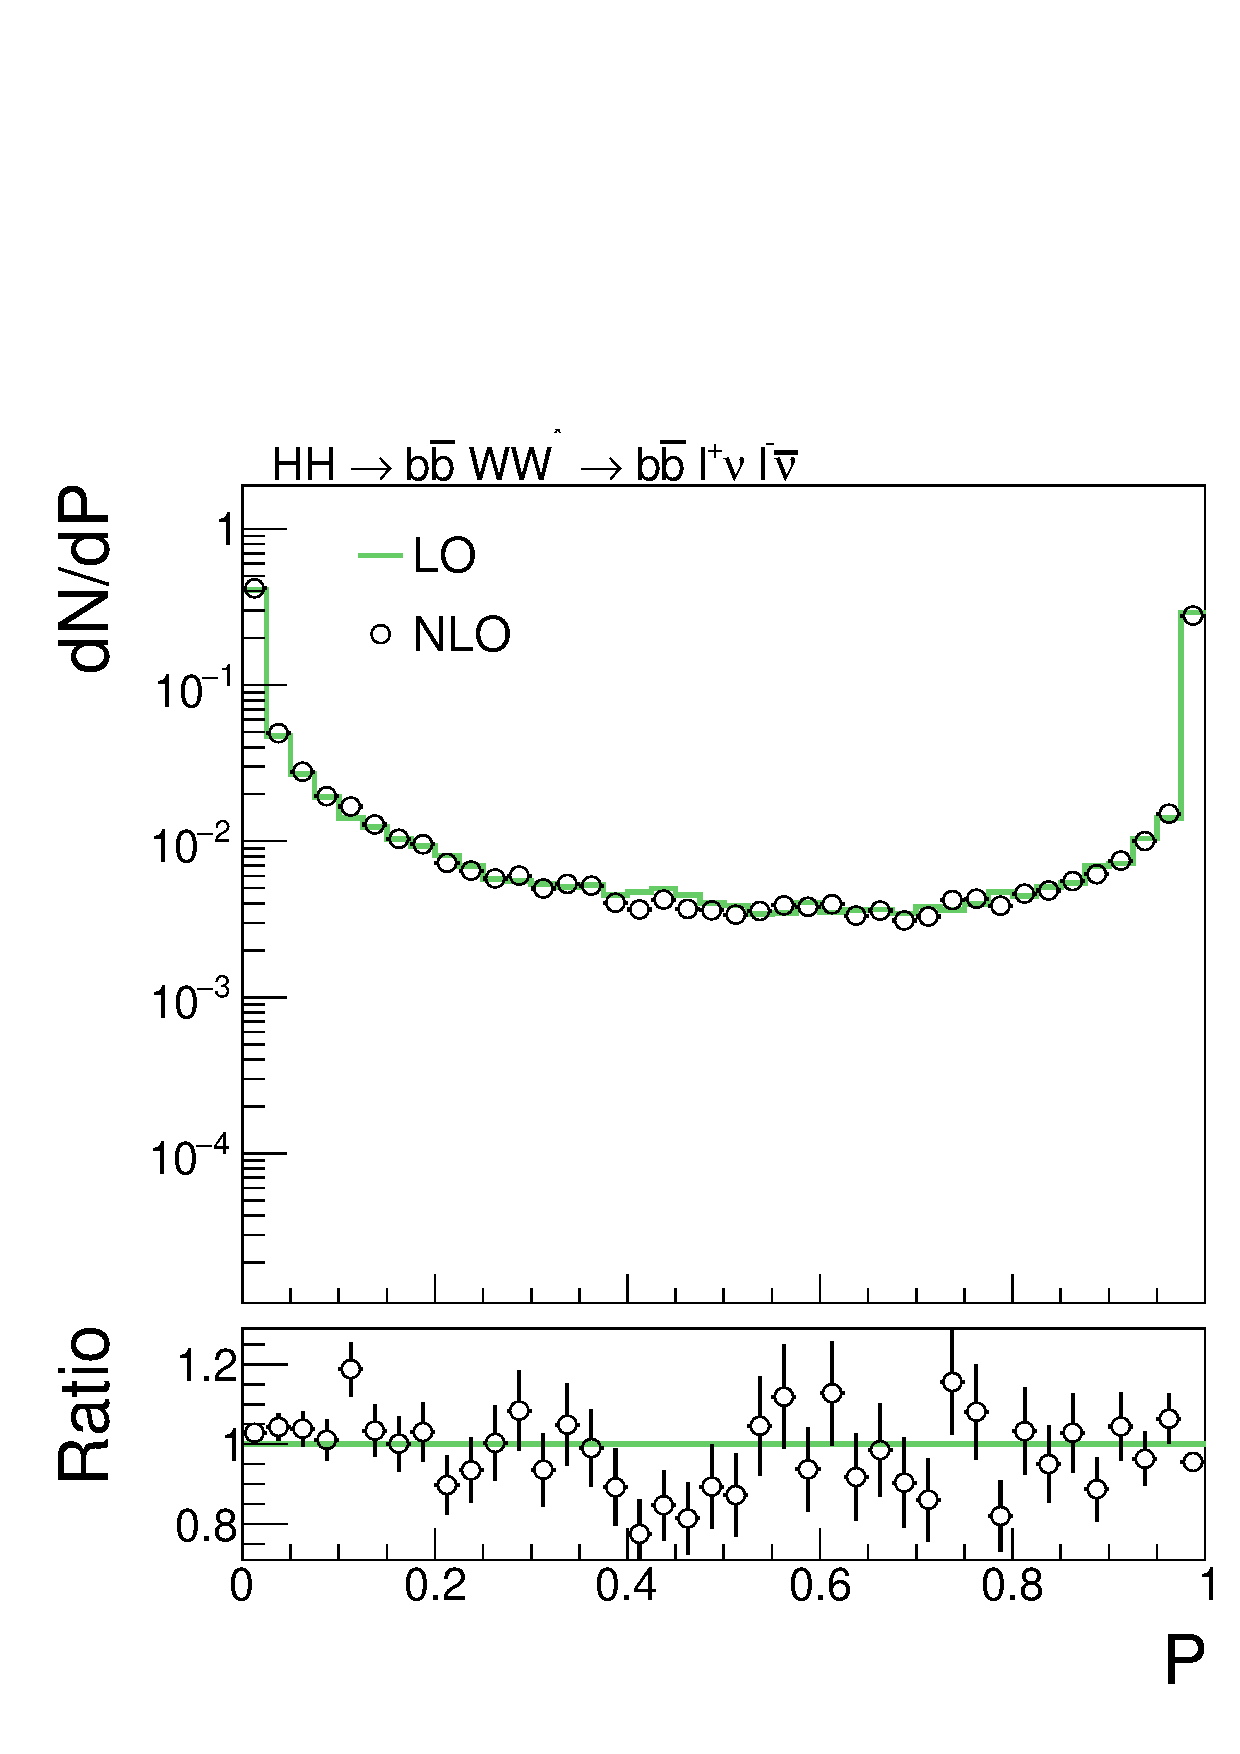
\includegraphics[width=0.48\textwidth]{plots/lo_vs_nlo_memLR_signal.pdf}
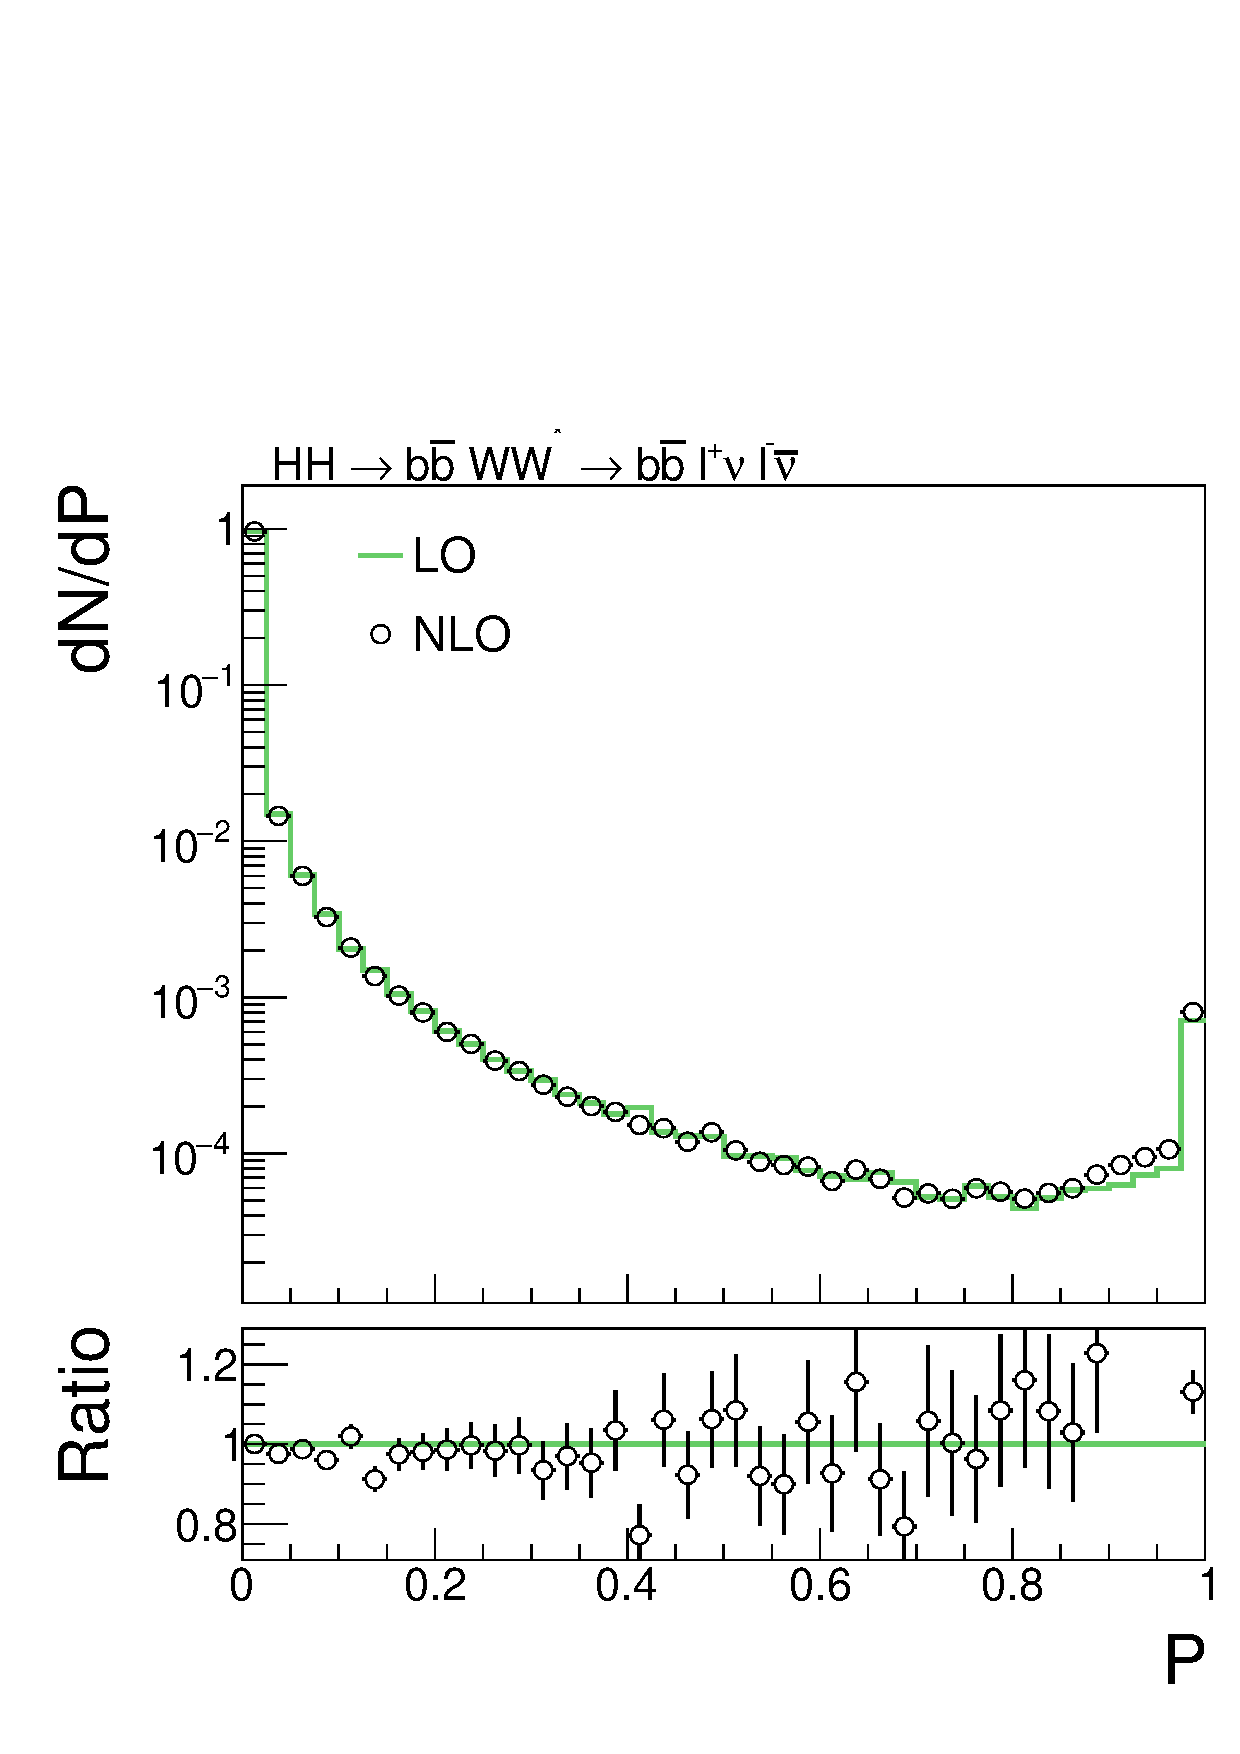
\includegraphics[width=0.48\textwidth]{plots/lo_vs_nlo_memLR_background.pdf}
\fi
\caption{
  Distribution in the LR $P(\vecy)$ 
  for $\dihiggs$ signal (left) and $\ttbar$ background (right) events
  simulated at LO and at NLO accuracy in pQCD.
  The likelihood ratios are computed at MC-truth level.
}
\label{fig:memLR_LO_vs_NLO}
\end{figure}

\begin{figure}
\ifx\ver\verPreprint
\setlength{\unitlength}{1mm}
\begin{center}
\begin{picture}(160,67)(0,0)
\put(39.5, 0.0){\mbox{\includegraphics*[height=67mm]
 {plots/lo_vs_nlo_ROC.pdf}}}
\end{picture}
\end{center}
\fi
\ifx\ver\verPAPER
\centering
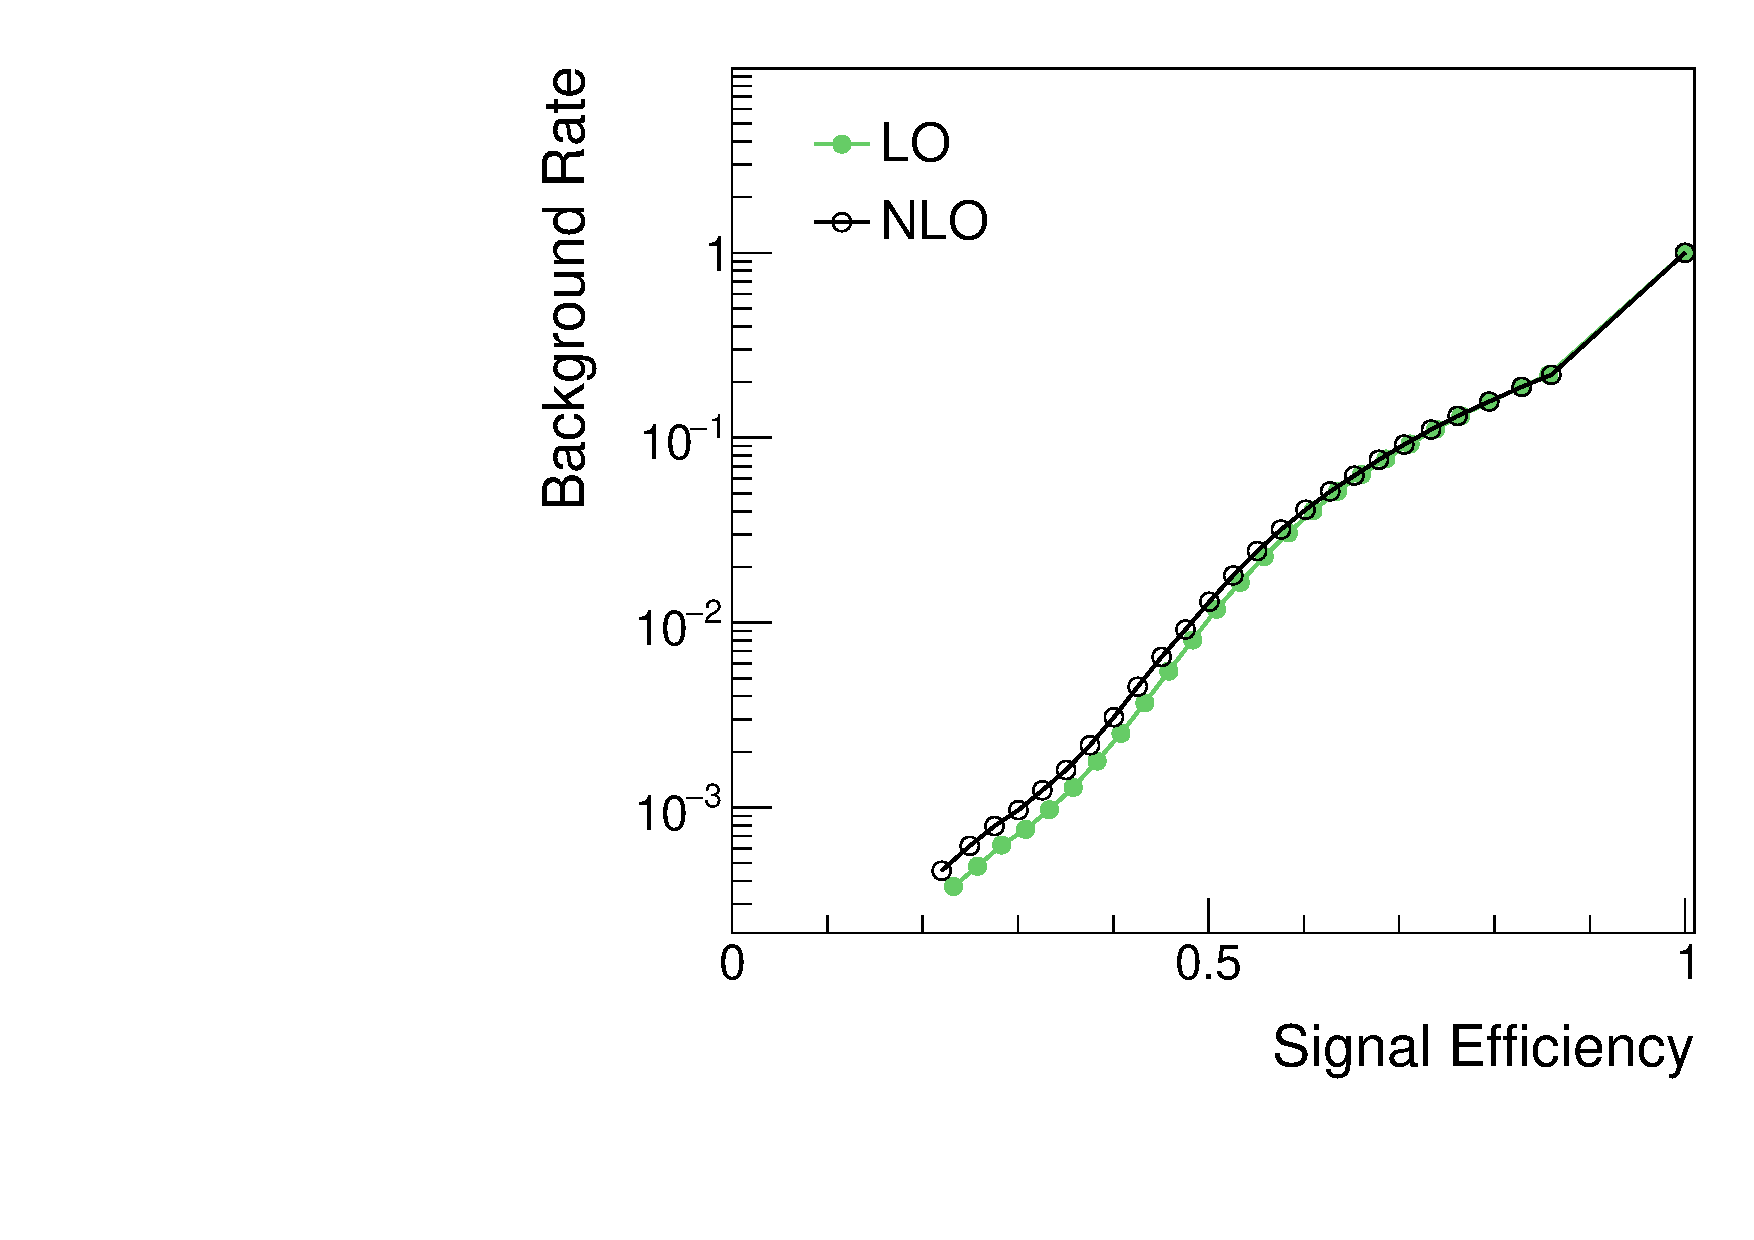
\includegraphics[width=0.48\textwidth]{plots/lo_vs_nlo_ROC.pdf}
\fi
\caption{
  Separation between the $\dihiggs$ signal and the $\ttbar$ background 
  for events simulated at LO and at NLO accuracy in pQCD.
  The graphs of background rate versus signal efficiency shown in the figure
  are obtained by applying a cut on the distributions in the likelihood ratios $P(\vecy)$ shown in Fig.~\ref{fig:memLR_LO_vs_NLO}.
}
\label{fig:ROC_LO_vs_NLO}
\end{figure}

The computing time required to evaluate the integrals given by Eqs.~(\ref{eq:mem_signal}) and~(\ref{eq:mem_background})
may represent a challenge in practical applications of the MEM.
Experimental analyses will usually need to evaluate these integrals
multiple times for each event in order to assess the effect of systematic uncertainties.
Taken together with the large cross section for $\ttbar$ production at the LHC,
the integrals in Eqs.~(\ref{eq:mem_signal}) and~(\ref{eq:mem_background}) may need to be computed in the order of $100$ million times.
Even with several thousands of computing jobs running in parallel,
as it is nowadays commonplace for experimental data analyses performed at the LHC,
the computation still requires a few weeks of nonstop computing time.
Several possibilities to speed up the numeric integrations, which take most of the computing time in practical applications of the MEM,
have been explored in the literature.
One alternative is to use vector integrands to evaluate the likelihood ratio for all systematic uncertainties simultaneously~\cite{CUBA},
taking advantage of the fact that the systematic uncertainties typically constitute small changes with respect to the nominal value.
Another alternative is to take advantage of the parallelizability of multidimensional integration and perform the integration on graphics processing units (GPUs).
Speedup factors of order $100$, compared to using a single core of a general-purpose central processing unit (CPU) 
such as the $2.30$~GHz Intel\TReg~Xeon\TReg~E5-2695V3 processor that we used for the studies presented in this paper,
are reported in the literature for performing numeric integrations on GPUs~\cite{Hagiwara:2009aq,Hagiwara:2009cy,Kanzaki:2010ym,Hagiwara:2013oka,Schouten:2014yza,Grasseau:2015vfa}.
